\documentclass[10pt,a4paper]{article}
\usepackage[T1]{fontenc}
\usepackage[utf8]{inputenc}
\usepackage[magyar]{babel}
\usepackage{graphicx}
\usepackage{subcaption}
\usepackage{float}
\usepackage{amsmath}
\usepackage{amsthm}
\usepackage{anysize}
\usepackage{bm}
\usepackage{physics}
\DeclareGraphicsExtensions{.pdf,.png,.jpg,.svg}
\linespread{1.3}
\numberwithin{equation}{subsection}
\numberwithin{figure}{section}
\bibliographystyle{plain}
\usepackage{hyperref}
\usepackage{environ}


\newtheorem{definition}{Definíció}[section]
\newtheorem{theorem}{Tétel}[section]

\newcounter{nextsec}
\newcommand\nextsection{%
  \setcounter{nextsec}{\thesection}%
  \stepcounter{nextsec}%
  \thenextsec%
}

\setlength\parindent{20pt}

\title{}

\newlength{\figurewidth}
\setlength{\figurewidth}{5cm}

\newenvironment{bfigure}[1]{\begin{figure} [#1] \begin{bf}}{\end{bf} \end{figure}}
\newcommand{\icaption}[1]{\caption{\textit{\textmd {#1}}}}
\newcommand{\colorg}[1]{{\color{green}{#1}}}


\NewEnviron{bigequation}{%
    \begin{equation}
    \scalebox{1.5}{$\BODY$}
    \end{equation}
    }


\begin{document}

\pagestyle{empty}


\begin{titlepage}

\center

\textsc{\LARGE  Eötvös Loránd Tudományegyetem}\\[0.5cm]
\textsc{\LARGE Természettudományi Kar}\\[0.5cm]
\textsc{\LARGE Fizikai Intézet}\\[1.5cm]
\vspace{8mm}

{ \huge \bfseries Háromrészecske Bose-Einstein korrelációk vizsgálata}\\[0.4cm] % Title of your document
\vspace{8mm}

\begin{center}
\LARGE \textit{Bagoly Attila}\\
\Large \textit{Fizikus MSc}\\
\end{center}

\begin{center}
\LARGE Témavezető: \\
\LARGE \textit{Csanád Máté}\\
\Large \textit{ELTE TTK Atomfizikai tanszék}\\
\end{center}
\vspace{4mm}



\begin{figure}[H] 
\centerline{ 

\includegraphics[height=5cm]{pic/ELTE_logo.png} 
} 
\end{figure}
\vspace{5mm}
\begin{Large}
\textbf{2017%. május 22.
}
\end{Large}

\begin{figure}[H]
\centering

\includegraphics[scale=0.03]{pic/CoulombCorrCode.png}
\end{figure}

\end{titlepage}

%\section*{Abstract}
%Bose-Einstein correlations of identical hadrons reveal information about hadron
%creation from the sQGP formed in ultrarelativistic heavy ion collisions. The
%measurement of three particle correlations may in particular shed light on
%hadron creation mechanisms beyond thermal/chaotic emission. In my work I'm measuring three pion correlations as a function of momentum
%differences within the triplets in RHIC PHENIX experiment. I analyzed the shape of these functions through the assumption
%of Levy sources and a proper treatment of the Coulomb interaction within the
%triplets. We determine Levy parameters scale ($R$), shape ($\alpha$) and three
%particle correlation strength ($\lambda_3$), where the latter, together with two
%particle correlation strength $\lambda_2$, encodes information about hadron
%creation mechanisms. From a consistent analysis of two- and three-particle
%correlation strength we are able to establish an experimental measure of the thermalization and coherence in the source.

\newpage
\tableofcontents

\clearpage
\pagestyle{plain}
\setcounter{page}{1}



\section{Bevezetés}

\subsection{Nagyenergiás nehézion-fizika}



A nehézion-fizikában nagy rendszámú atommagok közel fénysebességen való ütköztetésével próbálunk információt szerezni az elemi részecskék világáról. Az atommagokat közel fénysebességre gyorsítjuk elektromágneses terek segítségével (LHC, RHIC a két legnagyobb energiájú gyorsító). A labor-rendszerből nézve Lorentz-kontrahált atommagokat összeütköztetünk,  az ütközés során lejátszódnak bizonyos valószínűséggel ``kemény'' folyamatok amelyek során részecskezáporok (jet) keletkeznek, melyek hadronokból, leptonokból és fotonokból állnak. A kemény folyamatok jellemzője, hogy a jetek párokban keletkeznek, majd az impulzusmegmaradás miatt ellenkező irányba haladnak, az ütközések során a legvalószínűbb egy jet-pár keletkezése. Egy ütközés során nem csak kemény folyamatok zajlanak, hanem a ``lágy'' folyamatok is, melyek során a részecskék nem jetekben keletkeznek. Az ütköző atommagok tömegközépponti energiájának növelésével nő a kemény folyamatok valószínűsége, és csökken a lágy folyamatoké. Az ütközési pont köré épített detektorok segítségével mérjük a keletkező részecskék eloszlásait és különböző fizikai paramétereit. Ezen adatok segítségével próbálunk következtetni az ütközés után lezajló jelenségekre.

Az ütközések jellemzésére definiálni szoktuk az impakt paramétert, amely a középpontok távolságát jelenti. Az impakt paraméter alapján centralitás osztályokba rendezzük az ütközéseket, ezen osztályokat a centrálistól periférikus fele haladva százalékosan adunk meg.

Másik fontos fogalom a nukleáris módosulási faktor, amely segítségével az ütközés folyamatát tudjuk jellemezni. Az ütközés centralitását ismerve ki tudjuk számolni az ütközésben résztvevő nukleonok számát. A teljes folyamatot elképzelhetjük bináris ütközések összegeként, amennyiben feltesszük, hogy a protonok páronként ütköznek és egymástól függetlenül zajlanak az események. Független p+p ütközésekből ismerjük egy ilyen esemény során keletkező részecskék számát. Nehézion ütközések esetén ezt a számot megszorozzuk az ütközés bináris eseményeinek számával, így megkapjuk a keletkező részecskék számát. Azonban ezt a számot közvetlenül is meghatározhatjuk két nehézion összeütköztetésével, az előbbivel vett arányt nevezzük a nukleáris módosulási faktornak. Például Au+Au ütközés esetén, ha a keletkező részecskék száma $N_{{\rm Au}}$, bináris ütközések száma $N_{{\rm bin}}$ és p+p ütközések esetén a keletkező részecskék száma $N_{{\rm p}}$ akkor a nukleáris módosulási faktor a következőképpen néz ki:
\begin{large}
\begin{equation}
R_{\rm AA}=\frac{N_{\rm Au}}{N_{\rm bin}N_{\rm p}},
\label{eq:e1}
\end{equation}
\end{large}
ennek értékére  $R_{\rm AA}=1$ várunk, mivel az Au+Au ütközéseket úgy képzeljük el, hogy az ütközésben résztvevő protonok páronként ütköztek.  

\begin{center}
\begin{figure}[H]
\centering
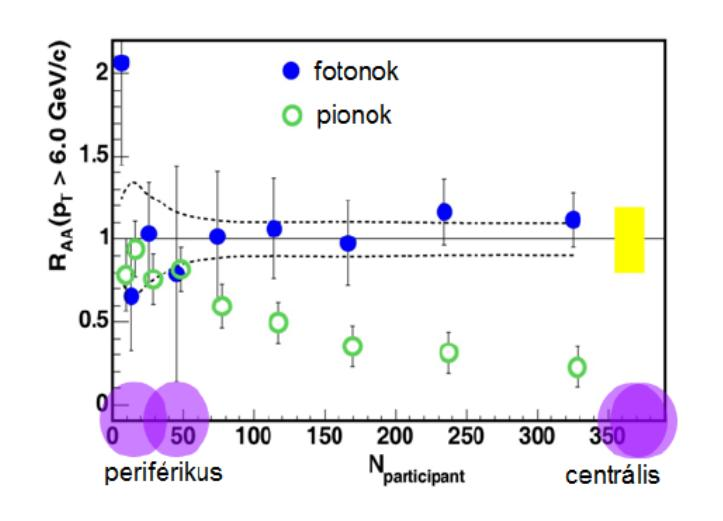
\includegraphics[scale=0.6]{pic/int/p1}
 \caption{Au+Au ütközések esetén a nukleáris módosulási faktor a nukleonszám függvényében pionokra és fotonokra. Az ábrán látható, hogy nagy centralitás esetén kevesebb nagyenergiás piont észlelünk mint p+p ütközések alapján várnánk, továbbá az erős kölcsönhatásban nem 
  fotonok száma a várttal egyezik. Ez utal az erősen kölcsönható közeg jelenlétére. Forrás: ~\cite{CsanadHabil}}
\label{fig:mmf}
\end{figure}
\end{center}

\subsection{Kvark-gluon plazma}

A RHIC gyorsítóban Au+Au ütközések során nagy nagy centralitásnál mérések során kevesebb nagyenergiás részecskét mértek a p+p ütközések alapján vártnál (\ref{fig:mmf} ábra), a jet-párok egyik tagja nem jelent meg. Azonban ezen tapasztalatoknak több kiváltó oka is lehet, a kérdés eldöntésére további kísérleteket végeztek. Az egyik volt a deutérium-arany ütközések elvégzése, azonban itt semmilyen centralitásnál nem volt jet-elnyomás. Ennek magyarázata, hogy ütközések esetén erősen kölcsönható közeg jöhet létre amely a jet-pár egyik tagját elnyeli (amely nagyobb utat tesz meg benne), azonban deutérium-arany ütközések során a létrejövő közeg mérete túl kicsi, hogy elnyelje azt.

Ezen közeg létrejöttét elméletileg a QCD magyarázza meg. Az elmélet szerint nagyon nagy energián megjelennek kvark szabadsági fokok, azaz a kvarkok hadronba zártsága megszűnik. A létrejövő közeg az erősen kölcsönható kvark-gluon plazma nevet viseli (sQGP). Ezen közegben nagyok a hatáskeresztmetszetek, ezért kicsi a szabad úthossz és gyors a termalizáció, ezért van értelme lokális egyensúlyról beszélni, így alkalmazhatóak rá a statisztikus fizika fogalmai (pl. hőmérséklet). Az ősrobbanást követő egy milliomod másodpercben az univerzumot is a kvark-gluon plazma alkotta ~\cite{SWeinberg}.

Az új közeg felfedezése után a RHIC gyorsítóban ezen közeg tulajdonságainak megismerését célzó kísérletek kezdődtek. Ezen kísérletek során kiderült, hogy a kvark-gluon plazma az eddig látott legtökéletesebb (viszkozitás mentes) folyadékként viselkedik, amely meglepő volt hisz nagyon kis viszkozitással rendelkező folyadékokat eddig nagyon alacsony hőmérsékleten tudtak csak előállítani. A kvarkfolyadék viszkozitására a gravitációs- és kvantumtérelméletek analógiájából (AdS/CFT) származik egy alsó becslés, eszerint a viszkozitás nem lehet kisebb mint $\hbar/4\pi$.

\begin{center}
\begin{figure}[H]
\centering
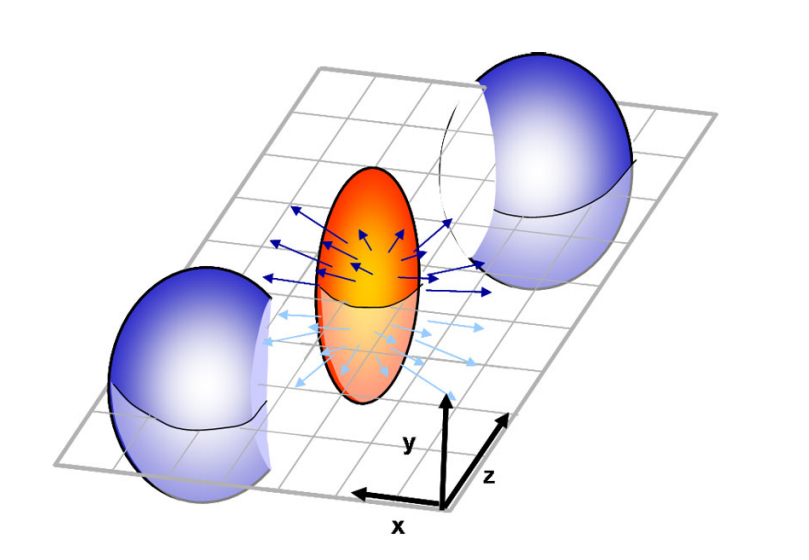
\includegraphics[scale=0.6]{pic/int/p2}
\caption{Két gömb ütközéseként létrejövő speciális ellipszoidális szimmetriával rendelkező kezdeti eloszlás kialakulása. Forrás: ~\cite{CsanadHabil}
}
\label{fig:ellip}
\end{figure}
\end{center}



Ultrarelativisztikus sebességre felgyorsított atommagok ütközése két Lorentz-kontrahált korong ütközéseként fogható fel, laborrendszerből nézve. Amint \aref{fig:ellip} ábra is szemlélteti, ez a létrejövő kvarkanyagban speciális kezdeti eloszlást eredményez, egy $\cos(2\varphi)$-szerinti aszimmetriát az eloszlásban, amely a tengelyszimmetriától való elliptikus eltérést jelenti.
A nyalábirányra merőlegesen bevezetjük a transzverz-síkot, ebben a síkban az kvarkanyag kezdeti eloszlását Fourier-sorba fejtjük a következőképpen:
\begin{large}
\begin{equation}
A(\varphi)= a_0+\sum_{n=1}^{\infty}\Big[a_n \cos(n\varphi)+b_n \sin(n\varphi)\Big]
\label{eq:e2}
\end{equation}
\end{large}
Ezen sorfejtés alapján látható, hogy az $a_2$ jellemzi az előbb említett aszimmetriát, amennyiben tökéletesen gömbszimmetrikusak lennének az atommagok és a keletkező ellipszis egyik nagytengelyén vennénk föl a a koordináta-rendszer x-tengelyét csupán ez a tag jelenne meg. Azonban mivel az atommagok véges nukleonszámmal rendelkeznek, melyeknek van valamilyen eloszlása a magon belül, a gömbszimmetria csupán első közelítésként fogható fel.

Az ütközés után létrejövő kvarkanyag robbanásszerűen tágul egész addig amíg a hőmérséklet le nem csökken egy bizonyos értékre, ekkor megszűnik ez a fázis és a kvarkokból hadronok keletkeznek amelyeket mérni is tudunk. Mivel a kvarkanyag folyadékszerűen viselkedik a kezdeti aszimmetriák nem tűnnek el, a kifagyás pillanatába is jelen vannak, ezért azok a keletkező hadronok eloszlásában is megjelennek. Az aszimmetriákat jellemző paramétereket az impulzustérben szokás definiálni. A részecskék eloszlását transzverz-síkban a $N(p_t, \varphi)$ függvénnyel jellemezzük, amely megmondja, hogy $[\varphi, \varphi+d\varphi]$ irányban $[p_t, p_t+dp_t]$ impulzus-tartományban mennyi részecske található. A függvény szögfüggését leválasztva, azt Fourier-sorba fejtve és 1-re normálva a következő alakban írhatjuk:
 \begin{large}
\begin{equation}
N(p_t, \varphi)= N(p_t)\bigg(1+\sum_{n=1}^{\infty}\Big[v_n \cos(n\varphi)+w_n \sin(n\varphi)\Big]\bigg)
\label{eq:e3}
\end{equation}
\end{large}
A Fourier-sor első komponensei játszanak fontosabb szerepet. Ezek közül is a $v_2$ együttható a leglényegesebb, mert ez a paraméter hordozza az ellipszoidális aszimmetriát, ezt az elliptikus folyás paraméterének nevezzük. Ezen aszimmetria a kifagyott hadronok és fotonok eloszlásában ~\cite{Adare:2011zr} is megjelenik, ezért a folyadékkép helyességét bizonyítja a kvark-gluon plazma esetén.
A Fourier-sor szinuszos részét nem szoktuk külön kezelni, mivel a mérések során a reakciósíkhoz képesti szög szerinti sort veszünk ($\sum v_n \cos[n(\varphi-\psi_n)])$, így a fenti szinuszos és koszinuszos tagok összevonva jelennek meg. Más mérési módszer esetén ugyan megjelenhetnek külön is a szinuszos tagok, de ekkor is szimmetria okokból ezen tagok eltűnnek.


\subsection{A PHENIX kísérlet}



\section{Bose-Einstein korrelációk}

Bose-Einstein korrelációk vizsgálatának megalapozói Robert Hanbury Brown és Richard Q. Twiss volt, ők 1956-ban publikált cikkükben ~\cite{HanburyBrown:1956bqd} vezették be a módszert, azonban munkájuk vegyes fogadtatásban részesült a tudományos közösség részéről. A módszer segítségével képesek voltak meghatározni a Sirius csillag átmérőjét a fotonok közötti korrelációk méréséből. Mérési elrendezésük két változtatható távolságra levő foton detektorból állt (ezek egy-egy fókuszáló tányér és fotoelektron-sokszorozóból álltak). A két detektor segítségével mérték a Sirius csillagból jövő fotonok közti korrelációt, különböző detektortávolságokon. Az így kapott pontokra elméleti megfontolásokból kapott korrelációs függvényt illesztettek, amely segítségével meghatározták a csillag átmérőjét. A két tudós tiszteletére a bozonok közti intenzitás korrelációt szokás Hanbury Brown és Twiss effektusnak nevezni (vagy röviden HBT effektus), az ilyen jellegű vizsgálódásokat pedig HBT analízisnek.

A HBT effektus részecskefizikai alkalmazásában jelentős szerepet játszott G. Goldhaber, S. Goldhaber, W.Y. Lee és A. Pais kutatása, akik proton-antiproton $1.05\;\mathrm{GeV/c}$ tömegközépponti energián történő ütköztetésekben keletkező pionokat vizsgáltak. Mérésük során azonos pionok között nem várt korrelációt tapasztaltak, melynek vizsgálatával felfedezték a $\rho^0$ rezonanciát, amely $4.5\cdot 10^{-24}$ másodperc alatt elbomlik két pionra ($\rho^0\rightarrow \pi^+\pi^-$), eredményüket 1960-ban publikálták ~\cite{Goldhaber:1960sf}. Később kiderült, hogy az általuk tapasztalt korrelációnak az oka, hogy a fotonokhoz hasonlóan a pionok is bozonok. Goldhaber és társai kutatása nyomán a részecskefizikában is beindult a HBT effektus vizsgálata. Későbbiekben kiderült, hogy az asztrofizikához hasonlóan ezek a korrelációk itt is információt hordoznak a forrás geometriájáról ~\cite{Padula:2004ba, CsanadHabil}. 


\subsection{Definíció}

Általánosan $n$ részecske közti korrelációs függvény a következőképpen definiálható ~\cite{Alt:1999cs, Csorgo:1999sj}:
\begin{equation}
C_n(p_1, p_2, \dots, p_n)=\frac{ N_n(p_1, p_2, \dots, p_n)  }{ N_1(p_1)N_1(p_2)\dots N_1(p_n)},
\label{eq:Cn}
\end{equation}
ahol $p_i=(p_i^0, \bm{p_i})$ 4-es impulzusmomentum, $ N_n(p_1, p_2, \dots, p_n)$ az $n$ részecske invariáns momentum eloszlás. A korrelációs függvény szemléletesen azt mondja meg, hogy milyen valószínűséggel keletkezik egy részecske n-es $p_1, p_2, \dots, p_n$ 4-es momentumokkal.

Az $n$ részecske invariáns impulzusmomentum eloszlás meghatározható a következő módon:
\begin{equation}
N_n(p_1, p_2, \dots, p_n) = \int \prod_{i=1}^{n}\mathcal{S}(p_i, x_i)\abs{\Psi_{p_1, {p_2}, \dots, {p_n}}({x_1}, {x_2}, \dots, {x_n})}^2\prod_{i=1}^{n}d^4 x_i,
\label{eq:Nn}
\end{equation}
ahol a $\Psi_{p_1, {p_2}, \dots, {p_n}}({x_1}, {x_2}, \dots, {x_n})$ az $n$ részecske hullámfüggvény, az $\mathcal{S}({p_i}, {x_i})$ pedig az úgynevezett forrásfüggvény, amely megadja annak a valószínűségét, hogy ${x_i}$ helyen keletkezik egy részecske ${p_i}$ impulzussal.

Az $n$ részecske hullámfüggvény meghatározásához nemrelativisztikus közelítést használunk HBT effektus vizsgálata során, így a függvényt a Schrödinger egyenlet megoldásából kapjuk (ügyelve, arra hogy mivel bozonjaink vannak, két részecske felcserélésére szimmetrikus legyen a hullámfüggvény):
\begin{equation}
i\hbar\frac{\partial \Psi(\bm{x_1},\dots, \bm{x_n},t )}{\partial t} = \Bigg[\sum_{i=1}^{n}\bigg(-\frac{\hbar^2}{2m_i}\Delta_i + V_i(\bm{x_i})\bigg) + \frac{1}{2}\sum_{i\neq j} V_{ij}(\bm{x_i},\bm{x_j})\Bigg]\Psi(\bm{x_1},\dots, \bm{x_n} ,t)
\label{eq:Sch0}
\end{equation}

A HBT effektus vizsgálatánál a különböző számítások könnyítése érdekében elhanyagoljuk az erős kölcsönhatást, amely tapasztalatok szerint pionok esetén megtehető, de már protonok esetén nem ~\cite{Pratt:1990zq}. Továbbá csak a párok közti Coulomb-kölcsönhatást vesszük figyelembe, elhanyagolva többi hadron által okozott töltésfelhőt. Így ~\aref{eq:Sch0} egyenlet a következő, egyszerűbb alakra egyszerűsödik:
\begin{equation}
i\hbar\frac{\partial \Psi(\bm{x_1},\dots, \bm{x_n},t )}{\partial t} = \Bigg[-\sum_{i=1}^{n}\frac{\hbar^2}{2m_i}\Delta_i + \frac{1}{2}\sum_{i\neq j} V_\mathcal{C}(\bm{x_i},\bm{x_j})\Bigg]\Psi(\bm{x_1},\dots, \bm{x_n} ,t)
\label{eq:Sch}
\end{equation}

Mivel energia saját állapotokkal dolgozunk, ezért  ~\aref{eq:Sch} egyenletet megoldó hullámfüggvény felírható:
\begin{equation}
\Psi_{p_1, {p_2}, \dots, {p_n}}(\bm{x_1},\dots, \bm{x_n},t )  
= \Psi_{\bm{p_1}, \bm{p_2}, \dots, \bm{p_n}}(\bm{x_1}, \bm{x_2}, \dots, \bm{x_n})\prod_{i=1}^ne^{-\frac{i}{\hbar}cp_i^0t},
\end{equation}
ahol $\Psi_{\bm{p_1}, \bm{p_2}, \dots, \bm{p_n}}(\bm{x_1}, \bm{x_2}, \dots, \bm{x_n})$ az időfüggetlen Schrödinger egyenlet megoldása:

\begin{equation}
\Bigg[-\sum_{i=1}^{n}\frac{\hbar^2}{2m_i}\Delta_i + \frac{1}{2}\sum_{i\neq j} V_\mathcal{C}(\bm{x_i},\bm{x_j})  
 - c\sum_{i=1}^n p_i^0
 \Bigg]\Psi_{\bm{p_1}, \bm{p_2}, \dots, \bm{p_n}}(\bm{x_1}, \bm{x_2}, \dots, \bm{x_n}) = 0
\end{equation}

Továbbá könnyedén belátható, hogy ~\aref{eq:Nn} egyenletben szereplő hullámfüggvény abszolút értéke szimmetrizációt elvégezve a következő lesz  (nemrelativisztikus közelítésben mondhatjuk, hogy $\bm{x_i} = (t,\bm{x_i})$) :
\begin{equation}
\abs{\Psi_{{p_1},{p_2}, \dots,{p_n}}({x_1}, {x_2}, \dots, {x_n})} = \frac{1}{\sqrt{n}}\abs{\sum_{(\alpha)}\Psi_{\bm{p_1}, \bm{p_2}, \dots, \bm{p_n}}(\bm{x_{\alpha_1}}, \bm{x_{\alpha_2}}, \dots, \bm{x_{\alpha_n}})}
\label{eq:Psin}
\end{equation}
ahol $\sum_{(\alpha)}$ az $(1,2,\dots,n)$ összes permutációjára való összegzés.


\subsection{Két nem kölcsönható részecske korrelációs függvénye}

Két azonos részecske esetén, nem kölcsönható esetben ~\aref{eq:Sch} egyenlet könnyedén megoldható, megoldásai a jól
ismert síkhullámok. A kétrészecskés invariáns impulzuseloszlásban szereplő hullámfüggvény szimmetrizáció
elvégzése után a következő lesz:
\begin{equation}
\Psi_{{p_1}{p_2}({x_1},{x_2})} = \frac{1}{\sqrt{2}}\big({e^{{ip_1x_1}+i{p_2x_2}}+e^{i{p_2x_1}+i{p_1x_2}}}\big)
\end{equation}

Tömegközépponti koordináta rendszerben, azaz a következő változókra való áttérés után (ezen transzformáció esetén az integrálási mérték nem változik, hiszen $d^4x_1d^4x_2=d^4Rd^4r$):
\begin{equation}
{K}={p_1+p_2},\;\;\;\;{k}=\frac{{p_1-p_2}}{2},\;\;\;\;{r}={x_1-x_2},\;\;\;\;{R}=\frac{{x_1+x_2}}{2}
\label{eq:CMF}
\end{equation}
\noindent
a hullámfüggvény abszolút értéke a következő alakra egyszerűsödik:
\begin{equation}
\abs{\Psi_{{p_1}{p_2}}({r},{R})} = \frac{1}{\sqrt{2}}\abs{e^{{KR}}(e^{i{kr}}+e^{-i{kr}})}=\sqrt{2}\abs{\cos{2{kr}}}
\end{equation}

Ebből következőleg a kétrészecske invariáns momentumeloszlásra a következő alak adódik):
\begin{equation}
N_2({p_1},{p_2})=\tilde{\mathcal{S}}(0, {p_1})\tilde{\mathcal{S}}(0, {p_2})+\frac{1}{2}\big(\tilde{\mathcal{S}}(2{k}, {p_1})\tilde{\mathcal{S^*}}(2{k}, {p_2})+\tilde{\mathcal{S^*}}(2{k},{ p_1})\tilde{\mathcal{S}}(2{k}, {p_2})\big),
\end{equation}
\noindent
ahol $\tilde{\mathcal{S}}$ a forrásfüggvény Fourier transzformáltja:
\begin{equation}
\tilde{\mathcal{S}}({q}, {k})=\int d^4x\mathcal{S}(x,k)e^{i{qx}}
\end{equation}

Az egyrészecske invariáns momentumeloszlásra pedig $N_1({p})=\tilde{\mathcal{S}}(0, {p})$ adódik. Ezekből ~\aref{eq:Cn} definíciót használva a kétrészecske korrelációs függvényre kapjuk a következő alakot:

\begin{equation}
C_2({p_1},{p_2}) = 1+ \frac{\tilde{\mathcal{S}}(2{k}, {p_1})\tilde{\mathcal{S^*}}(2{k}, {p_2})+\tilde{\mathcal{S^*}}(2\bm{k},{ p_1})\tilde{\mathcal{S}}(2\bm{k}, {p_2})}{2\tilde{\mathcal{S}}(0, {p_1})\tilde{\mathcal{S}}(0, {p_2})}
\end{equation}

Szokás alkalmazni a ${p_1}\approx {p_2}\approx {K} = p_1+p_2$ közelítést ($q\ll K$), amelyet az indokol, hogy a  forrást Fourier transzformáltjának az egyes részecskék momentumától való függése sokkal simább mint a relatív momentumtól való függése ~\cite{Lisa:2005dd}. A kétrészecske korrelációs függvény ekkor: 
\begin{equation}
C_2({k}, {K})=1+\frac{\abs{\tilde{\mathcal{S}}({k},{K})}^2}{\abs{\tilde{\mathcal{S}}(0,{K})}^2}
\label{eq:C02}
\end{equation}

Ez az alak azt a fontos üzenetet hordozza, hogy a kétrészecske korrelációs függvény meghatározásával megkapjuk a forrásfüggvény Fourier transzformáltját. Tehát a korrelációs függvény méréssel a forrás függvényt meg tudjuk határozni. 


A korrelációs függvény a $k,K$ négyes impulzusok helyett hármas momentumokkal is kifejezhető, ugyanis a két négyesmomentum szorzata definíció és az egyes részecskék tömeghéj feltétele ($p_{i\mu}p^{\mu}_i=0$) alapján eltűnik, azaz:
\begin{equation}
0=kK=k_0K_0-\bm{kK}\Rightarrow k_0 = \frac{\bm{kK}}{K_0}
\end{equation}

A $p_1\approx p_2\approx K$ feltevés alapján a $K$ körülbelül tömeghéjon van, azaz $K_0 = \sqrt{m^2-\bm{K}^2}$, így a korrelációs függvény a $k,K$ négyes-momentumok helyett a $\bm{k},\bm{K}$ hármas-momentumok függvényeként is tekinthető.

\subsection{Forrás függvény}
~\Aref{eq:Nn} egyenletben szereplő $\mathcal{S}({p},{x})$ függvényt nevezzük forrásfüggvénynek, ez megadja annak a valószínűségét, hogy ${x}$ helyen keletkezik egy ${p}$ impulzusú részecske. Az általunk vizsgált energiákon, az ütközés során kvark-gluon plazma keletkezik, amely robbanásszerűen tágul, melynek következtében csökken a hőmérséklete. Ha lokálisan a QGP elér egy bizonyos hőmérsékletet, akkor fázisátmenet történik, kifagynak a kvark szabadsági fokok és hadronok keletkeznek. A forrásfüggvényt épp ezen fázisátmenetek határozzák meg. 

A fázisátmenetet pillanatszerűnek tekinthetjük, mivel ha feltesszük, hogy ez nem teljesül, akkor mondhatjuk, hogy a forrásfüggvény felírható szorzat alakban: $\mathcal{S}({x}) = \mathcal{S}_T(\tau)\mathcal{S}(\bm{x})$. Az időfüggő részre feltehető továbbá (\cite{CsanadHabil}):
\begin{equation}
\mathcal{S}_T(\tau)=\frac{1}{(2\pi \Delta\tau)^\frac{3}{2}}e^{-\frac{(\tau-\tau_0)^2}{2\Delta\tau^2}}
\end{equation}

Térszerű részre kevés megszorítással élve, a kétrészecske korrelációs függvényre a következő alak adódik (\cite{CsanadHabil}):
\begin{equation}
C_2(k)=1+\lambda e^{-k_0\Delta\tau^2-k_{\mathrm{long}}R_{\mathrm{long}}^2-k_{\mathrm{side}}R_{\mathrm{side}}^2-k_{\mathrm{out}}R_{\mathrm{out}}^2},
\end{equation}
ahol az $R_{\mathrm{long}},R_{\mathrm{side}},R_{\mathrm{out}}$ az úgynevezett HBT sugarak. Továbbá adódik a HBT sugarak közti következő összefüggés (\cite{CsanadHabil}):
\begin{equation}
R_{\mathrm{out}}^2-R_{\mathrm{side}}^2\propto \Delta\tau^2
\end{equation}

Kísérleti tapasztalat továbbá, hogy $R_{\mathrm{out}}\approx R_{\mathrm{side}}$, ebből következőleg a $\Delta\tau\approx 0$, tehát, a  forrásfüggvény időfüggő része egy $\tau_0$-ra koncentrált Dirac-delta, azaz a fázisátmenet pillanatszerűen történik ~\cite{Ster:2010ia, Csorgo:1999sj, Csanad:2009wc}.

%~\Aref{eq:Psin} egyenletnél láttuk, hogy az invariáns momentum eloszlásban megjelenő hullámfüggvény időfüggetlen.


A forrásfüggvény alakjára elsődlegesen Gauss eloszlást alkalmaztak ~\cite{Csorgo:2005gd, Lisa:2005dd}, azonban a PHENIX kísérletben $\sqrt{s_{NN}}=200\;\mathrm{GeV}$ tömegközépponti energiájú arany-arany ütközések során bizonyítékot találtak nem gaussi, lassan lecsengő struktúrára ~\cite{Adler:2006as}. Egy magyarázat a lassan lecsengő viselkedésre lehet a Lévy repülés ~\cite{Csanad:2007fr}. A kvark-glon plazmából már kifagyott hadronok gáza tágul, így a rendszer egyre hidegebb, ritkább lesz, a hatáskeresztmetszetek egyre kisebbé válnak, megnövelve az átlagos szabad úthosszat. Ennek következtében egyre hosszabb lépések is megjelennek a hadronok véletlen bolyongás során. Ennek következtében eltávolodás eloszlása lassan lecsengő eloszlás lesz, melynek szórása már nem létezik. Ezen véletlen bolyongó hadronok aztán elbomolhatnak a vizsgált részecskékre, ezért járulékot adnak a forrásfüggvénybe. Ezen hadronok eltávolodása (QGP-ből való kifagyás helyétől), a centrális határeloszlás tétele alapján Lévy eloszláshoz tart, hiszen az összeadott lépések lassan lecsengő eloszlással rendelkező valószínűségi változónak tekinthető.

\subsubsection{Lévy eloszlás}

A forrásfüggvény alakjára munkám során három dimenziós Lévy eloszlást használtam. A Lévy eloszlás három dimenzióban a következő karakterisztikus függvény segítségével adható meg:
\begin{equation}
\Phi(\bm{q}, \alpha, R) = e^{-\abs{\bm{q}R}^\alpha}
\end{equation}
A karakterisztikus függvény Fourier transzformáltját kiszámolva (az integrálás csak numerikusan végezhető el) megkapható a Lévy eloszlás:
\begin{equation}
\mathcal{L}(\bm{r},\alpha,R) = \frac{1}{(2\pi)^3}\int d^3q \Phi(\bm{q}, \alpha, R)e^{i\bm{qr}}= \frac{1}{(2\pi)^3}\int e^{i\bm{qr}}e^{-\abs{\bm{q}R}^\alpha},
 \label{eq:Levyint}
\end{equation}
\noindent
ahol $0< \alpha \leq 2$ és $0<R$ a Lévy eloszlás paraméterei. Speciálisan, $\alpha=2$ esetén a Lévy eloszlás a normális eloszlás lesz:
\begin{equation}
\mathcal{N}(\bm{r},\sigma) = \mathcal{L}\bigg(\bm{r}, \frac{\sigma}{\sqrt{2}}\bigg) = \mathcal{L}\big(\bm{r}, 2^{-\frac{1}{\alpha}}\sigma\big)
\end{equation}

Mivel Lévy eloszlást használunk a forrás modellezésére, ezért a Lévy paraméterek a forrásról hordoznak információt, és magára a forrásra jellemzőek. Egy $\alpha, R$ paraméterű forrás esetén, a forrásfüggvényre a következő alakot használjuk:
\begin{equation}
\mathcal{S}(p,x; \alpha, R) =\mathcal{L}\big(\bm{x}, \alpha, 2^{-\frac{1}{\alpha}}R\big)
\end{equation}

A Lévy eloszlás skálaparamétertől való függésére ($R$ paraméter) teljesül a következő összefüggés:
\begin{equation}
\mathcal{L}(\bm{r}, \alpha, R) = \mathcal{L}\bigg(\frac{\bm{r}}{R}, \alpha, 1\bigg)R^{-3}\equiv \mathcal{L}\bigg(\frac{\bm{r}}{R}, \alpha\bigg)R^{-3}
\end{equation}

Továbbá az eloszlás nem függ az $\bm{r}$ irányától, csak a nagyságától (belátható változócsere segítségével $\bm{q'}=\bm{Aq}$: $\abs{\bm{q}}=\abs{\bm{q'}}\bm{qr}=\abs{\bm{q}}\abs{\bm{r}}$, ekkor $d^3 q=d^3 q'$):
\begin{equation}
\mathcal{L}(\bm{r}, \alpha, R)=\mathcal{L}(\abs{\bm{r}}, \alpha, R)
\end{equation}

Az egydimenziós Lévy eloszlás aszimptotikus viselkedéséből  ~\cite{LevyEff} kiindulva könnyedén meghatározható a háromdimenziós eloszlás viselkedése is. Nagy $r$ paraméter esetén, a Lévy eloszlás a következő sor segítségével kapható meg ($r>>1$):

\begin{equation}
\mathcal{L}(r,\alpha) \approx \frac{\alpha}{2\pi^2}\sum_{k=1}^{N}(-1)^{k+1}\frac{\Gamma(\alpha k)}{\Gamma(k)} \sin{\bigg(\frac{\pi\alpha k}{2}\bigg)}\frac{\alpha k+1}{r^{\alpha k+3}},
\end{equation}
ahol $\Gamma(x)$ a Gamma függvény:
\begin{equation}
 \Gamma (z)=\int _{0}^{\infty }x^{z-1}e^{-x}\,dx
 \label{eq:gamma}
\end{equation}

A kis $r$ viselkedés hasonló módon egy sor segítségével kapható ($r<<1$):
\begin{equation}
\mathcal{L}(r,\alpha) \approx -\frac{1}{2\pi^2\alpha}\sum_{k=0}^n\frac{\Gamma\big(\frac{k+3}{\alpha}\big)}{\Gamma(k+3)}\sin{\bigg(\frac{\pi(k+3)}{2}\bigg)}(k+2)(k+1)x^k
\end{equation} 

A Lévy eloszlás meghatározása során kis és nagy értékekre ezen aszimptotikus sorokat alkalmaztam, a köztes tartományban pedig 15 pontú adaptív Gauss Kronrod integrálási módszert alkalmaztam (részletek \aref{sec:GK} fejezetben), melyet GPU-ra párhuzamosítva CUDA-ban (részletek \aref{sec:CUDA} fejezetben), továbbá klasztere párhuzamosítva MapReduce programozási modellben implementáltam (részletek \aref{sec:MapReduce} fejezetben). Az integrálást sok paraméterre elvégeztem (felbontást úgy állítottam be, hogy két pont között lineáris interpoláció hibája a megengedett hiba alatt legyen), eredményekből egy Lévy táblázat készült, amelyhez egy könnyen használható olvasó interfész tartozik. Néhány $\alpha$ és $R$ paraméter esetén az eloszlást \aref{fig:Levy} ábrák szemléltetik.

\begin{figure}[H]
\centering
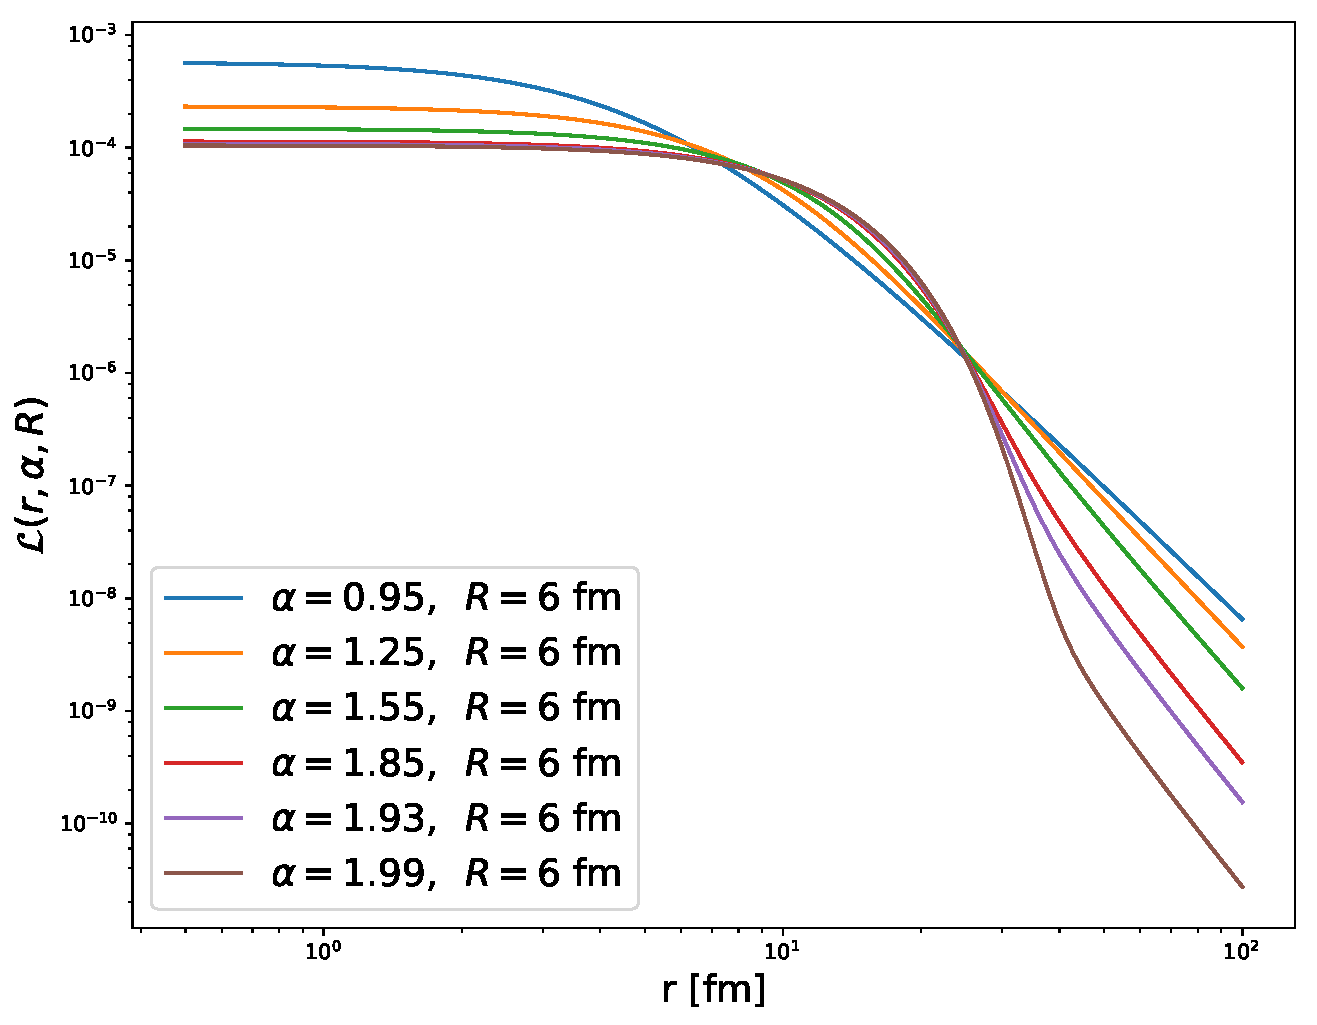
\includegraphics[scale=0.35]{pic/BEintro/Levy_alpha.pdf}
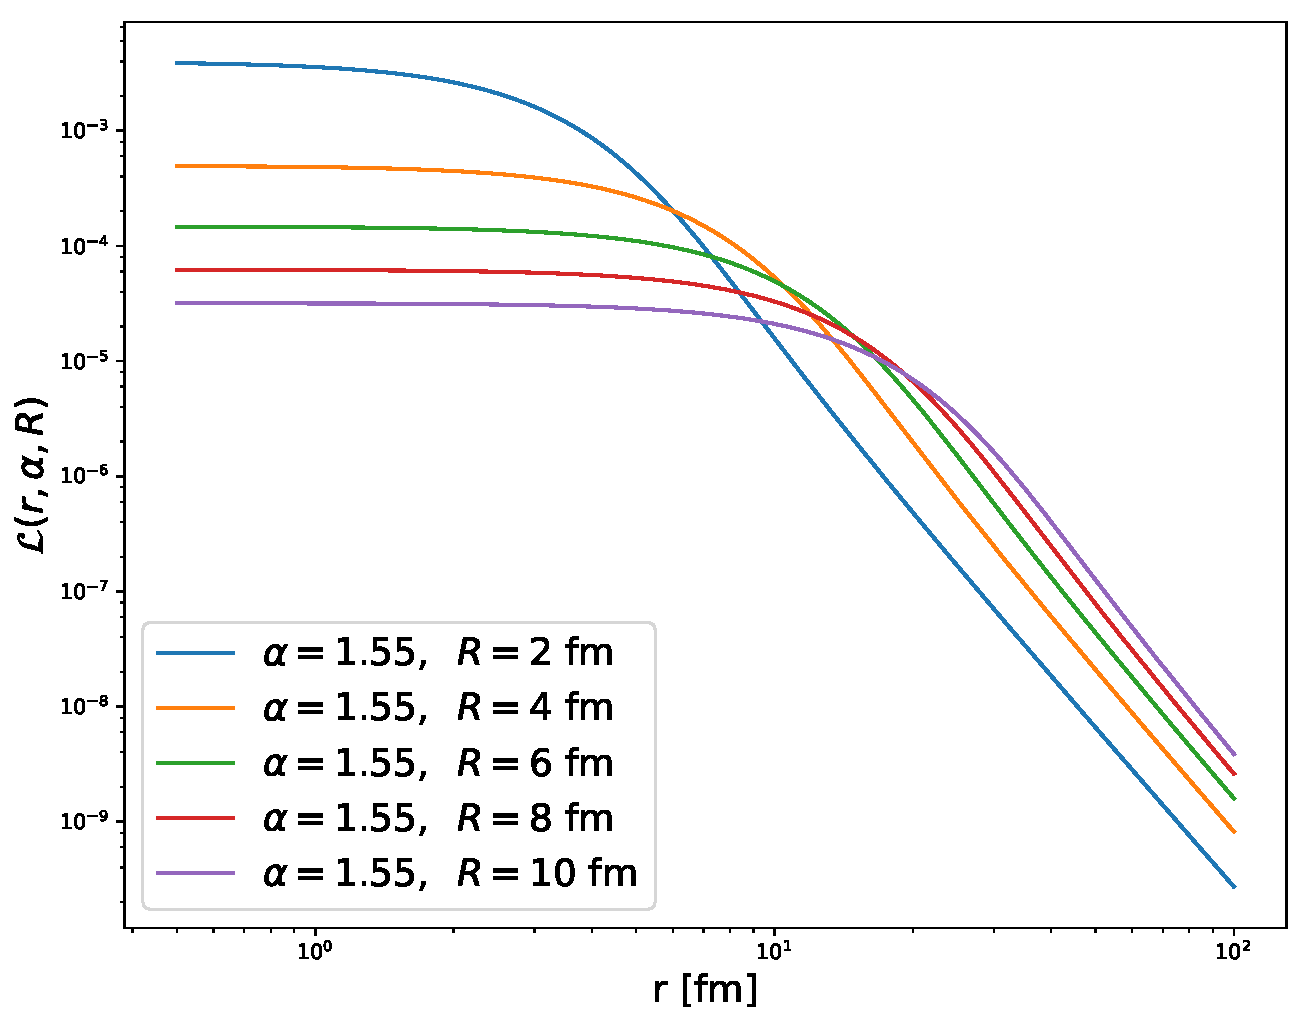
\includegraphics[scale=0.35]{pic/BEintro/Levy_R.pdf}
\caption{Háromdimenziós Lévy eloszlás sugárfüggése különböző $\alpha$ és $R$ paraméterek esetén.}
\label{fig:Levy}
\end{figure}

\subsection{A mag-glória modell}
A HBT effektus vizsgálata során nehéz ionokat ütköztetünk nagy energián. Az ütközés során létrejövő kvark-gluon plazma robbanásszerűen tágul (ezen tágulás leírására hidrodinamika alkalmazható), elérve egy kritikus hőmérsékletet fázisátmenet történik, hadronok fagynak ki pillanatszerűen. A hadronok közül munkánbana  töltött pionok közti korrelációt vizsgáltam, mivel ezen részecskékből keletkezik a legtöbb az ütközések során. A kirepülő pionokat az ütközési centrum köré épített detektorrendszerrel detektáljuk. Azonban pionok nem csak a forró kvarkanyag kifagyása során  keletkeznek, hanem később, instabil részecskék (pl. $\eta,\eta',\omega$) bomlásából is ~\cite{Bolz:1992hc}. Ezen jelenség leírására szolgál a mag-glória (core-halo) modell ~\cite{Csorgo:1994in,Csorgo:1999sj}, melynek szemléltetése ~\aref{fig:ch1} ábrán látható. A mag mérete $10$ femtométer alatti, míg a glória mérete több száz, vagy akár több ezer femtométer is lehet, mivel egyes hosszú élettartamú instabil részecskék ilyen távolságokra jutnak el mielőtt elbomlanának pionokra.
\begin{figure}[H]
\centering
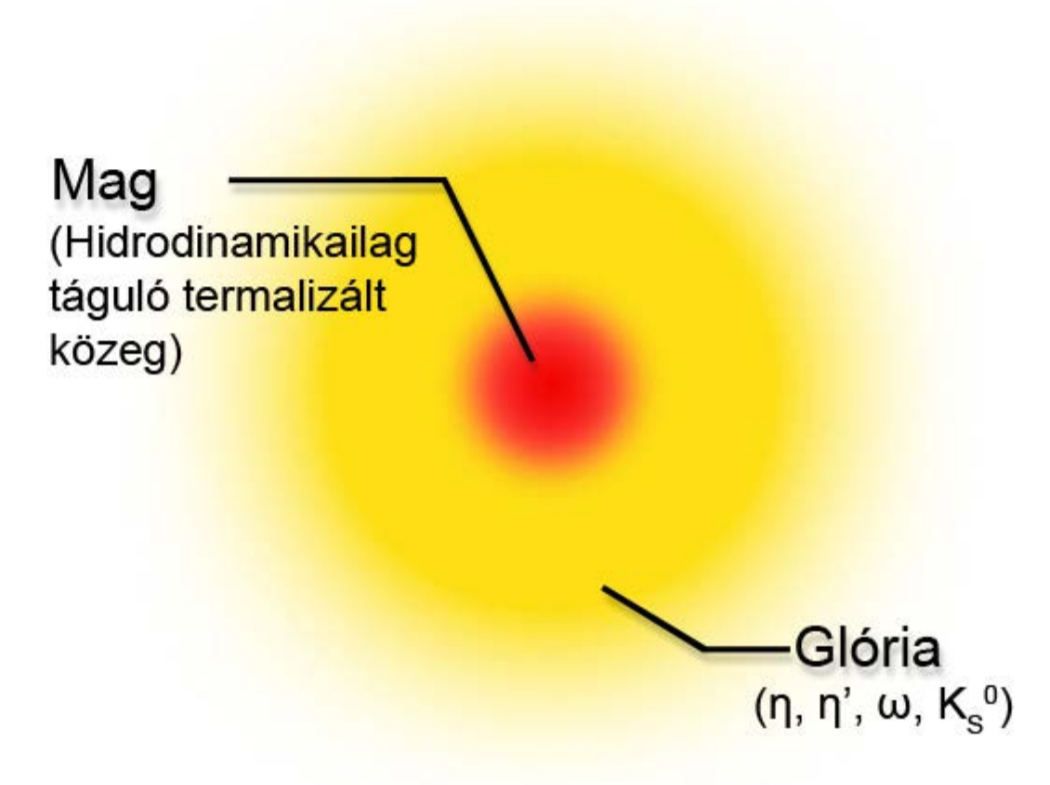
\includegraphics[scale=0.5]{pic/BEintro/CH1}
\caption{Mag-glória modell szemléltetése. Forrás \cite{Kofarago}}
\label{fig:ch1}
\end{figure}

Mivel ~\aref{eq:C02} összefüggés alapján a korrelációs függvény a forrás Fourier transzformáltjával áll kapcsolatban, továbbá a glóriában a pionok nagy $x$ távolságokon keletkeznek, ezért a glória  kis relatív impulzusú tartományban ad járulékot a korrelációs függvényhez. Ugyanakkor a detektor impulzusfelbontása véges, ezért az egymáshoz nagyon közeli impulzussal rendelkező részecskék nem megkülönböztethetőek, azaz bizonyos relatív impulzus alatti tartományban (felbonthatatlan régió) nem tudjuk megmérni a korrelációs függvényt. Ezt az effektust szemlélteti ~\aref{fig:ch2} ábra.

A mag-glória modellben feltételezünk egy magot valamint egy glóriát leíró forrásfüggvény lététezését. A teljes rendszert leíró forrásfüggvény pedig ezen kettő összege:
\begin{equation}
\mathcal{S}(x,p)=\mathcal{S}_M(x,p)+ \mathcal{S}_G(x,p)\Longrightarrow \mathcal{\tilde{S}}(k, K) = \mathcal{\tilde{S}}_M(k,K)+\mathcal{\tilde{S}}_G(k,k)
\end{equation}

Mivel a Fourier transzformált a nulla helyen megegyezik a függvény integráljával, továbbá a forrásfüggvény integrálja a keletkezett részecskék számát adja meg, ezért ha a magban keletkező részecskék száma $N_M$, a glóriában $N_G$, akkor:
\begin{equation}
\mathcal{\tilde{S}}_M(0,K) = N_M,\;\;\;\;\; 
\mathcal{\tilde{S}}_G(0,K) = N_G,\;\;\;\;\;
\mathcal{\tilde{S}}(0,K) = N_M+N_G
\end{equation}

A nagy (legalább $50$ fm) szélességű $\mathcal{S}_G$ keskeny $\mathcal{\tilde{S}}_G$ Fourier transzformáltat eredményez, melynek  szélessége maximálisan $4$ MeV. Ez a maximális szélesség a detektor véges felbontóképességéből adódó felbonthatatlan régióba esik tipikusan, ezért az mondható, hogy: $\mathcal{\tilde{S}}_G\approx 0$, azaz $\mathcal{\tilde{S}}=\mathcal{\tilde{S}}_M$. Ebből a kétrészecske korrelációs függvényre adódik:
\begin{equation}
C_2({k}, {K})=1+\frac{\abs{\tilde{\mathcal{S}}({k},{K})}^2}{\abs{\tilde{\mathcal{S}}(0,{K})}^2} =
1+\frac{\abs{\tilde{\mathcal{S}}_M({k},{K})}^2}{\Big(N_M+N_G\Big)^2}
 =
  1+\lambda_2\frac{\abs{\tilde{\mathcal{S}}_M({k},{K})}^2}{\abs{\tilde{\mathcal{S}}_M(0,{K})}^2},
\end{equation}
ahol bevezettem a:
\begin{equation}
\lambda_2=\frac{N_M^2}{\Big(N_M+N_G\Big)^2} \equiv f_C^2
\label{eq:CHlambda2}
\end{equation}
jelölést. Az összefüggésben bevezettem egy új mennyiséget, a mag arányt arányát, amely megmondja, hogy az összes észlelt részecske, hányad része származik a magból:
\begin{equation}
f_C=\frac{N_M}{N_M+N_G}
\label{eq:fC}
\end{equation}

Tehát amíg ~\aref{eq:C02} egyenletben a $k\rightarrow 0$ esetben a korrelációs függvény $C_2(k,K)\rightarrow 2$, addig mag-glória modellben, a $2$ helyett a $1+\lambda_2$-höz tart a korrelációs függvény.

\begin{figure}[H]
\centering
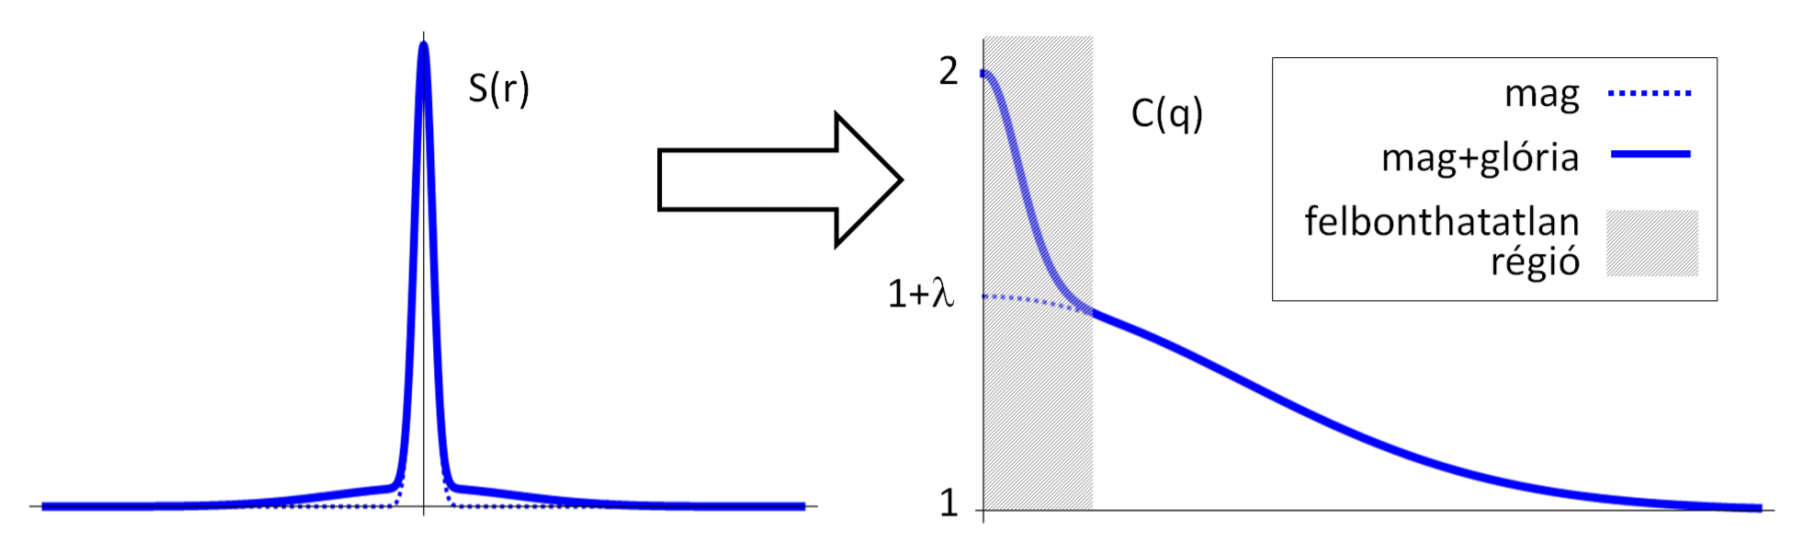
\includegraphics[scale=0.4]{pic/BEintro/CH2}
\caption{Keskeny magból és széles glóriából álló forráshoz tartozó korrelációs függvény. A glória keskeny csúcsot eredményez a korrelációs függvényben, amely a detektor véges felbontásának következtében nem látható. Forrás: ~\cite{CsanadHabil}}
\label{fig:ch2}
\end{figure}


\subsection{A korreláció erőssége}
A mag-glória modellnél láttuk, hogy a kétrészecske korrelációs függvény kis relatív impulzusokra tart ~\aref{eq:CHlambda2} egyenlet által definiált $\lambda_2$ paraméter által meghatározott $1+\lambda_2$ értékhez. Ezt a paramétert szokás kétrészecske korrelációs erősségnek nevezni.

Ebből kiindulva általánosan definiálhatjuk az $n$ részecske korrelációs erősséget:
\begin{equation}
\lambda_n = \lim_{k_1\rightarrow 0}\dots\lim_{k_n\rightarrow 0}C_n(k_1,\cdots,k_n)-1
\label{eq:lambdan}
\end{equation}

Mag-glória modell esetén az $n$ részecske korrelációs erősség kifejezhető ~\aref{eq:fC} összefüggéssel definiált magarány segítségével a következőképpen ~\cite{Csorgo:1997uf}:
\begin{equation}
\lambda_n =\sum_{j=1}^n\binom{n}{j}\alpha_j f_C^j
\label{eq:CHlambdan}
\end{equation}

Az egyenletben szereplő $\alpha_j$ paraméter a következőképpen határozható meg:
\begin{equation}
\alpha_n = n!-1-\sum_{j=1}^{n-1}\binom{n}{j}\alpha_j,
\label{eq:alphan}
\end{equation}
első néhány értéke: $\alpha_1=0,\;\alpha_2=1\;\alpha_3=2$.

\subsection{Parciális koherencia}

Az eddigiekben feltettük, hogy a forrás teljesen kaotikus, a kifagyott pionok fázisa teljesen véletlenszerű. Azonban előfordulhat, hogy a kifagyott részecskepárok fáziskülönbsége részben állandó, azaz a forrás részben koherens módon kelt részecskéket. Ezt az effektust nevezik parciális koherenciának ~\cite{Csorgo:1998tn, Csorgo:1999sj, Csorgo:1997uf}. Ekkor a momentum eloszlást másképp kell számolni, hiszen ~\aref{eq:Nn} összefüggésben már kihasználtuk, hogy a részecskék fázisa véletlenszerű, melynek következtében átlagolás során eltűnik. 

Az effektust mag-glória modellnél látottakhoz hasonló módon történő figyelembevétele érdekében bevezetjük a koherencia arányát, amely megadja, hogy a magból származó részecskék hányad része keletkezett koherens módon:
\begin{equation}
p_C = \frac{N_M^C}{N_M}
\end{equation}

Mag-glória modellnél láttuk, hogy amennyiben a részecskék nem csak közvetlenül a forró kvarkanyagból származnak, akkor az $n$ részecske korrelációs erősségek függeni fognak ~\aref{eq:fC} egyenlet által definiált magaránytól ~\aref{eq:CHlambdan} egyenlet által meghatározott módon. Ehhez hasonlóan, azt mondhatjuk, hogy amennyiben részecske keletkezés során van parciális koherencia, akkor az $n$ részecske korrelációs erősség függeni fog a magarány mellett a koherencia arányától a következő módon ~\cite{Csorgo:1998tn, Csorgo:1997uf}:

\begin{equation}
\lambda_n(f_C, p_C) = \sum_{j=2}^{n}\binom{n}{j}\alpha_j f_C^j\big[(1-p_C)^j+jp_C(1-p_C)^{j-1}\big],
\end{equation}
ahol az $\alpha_j$ paramétert ~\aref{eq:alphan} egyenlet határozza meg. Az egyenlet két- és háromrészecske esetén a következőkre egyszerűsödik:

\begin{equation}
\lambda_2 =  f_C^2\big[(1-p_C)^2+2p_C(1-p_C)\big]
\end{equation}

\begin{equation}
\lambda_3 =  2f_C^3\big[(1-p_C)^3+3p_C(1-p_C)^2\big]+3f_C^2\big[(1-p_C)^2+2p_C(1-p_C)\big]
\end{equation}

Ezen két egyenlet mutatja, hogy két- és háromrészecske korrelációk vizsgálatából amennyiben meghatározzuk a korrelációs erősségeket, meghatározható az $f_C$ és $p_C$ paraméter, azaz a magból származó részecskék aránya, illetve a magban koherens módon keletkezett részecskék aránya.

Koherencia létének vizsgálata érdekében vezessük be a következő paramétert:
\begin{equation}
\kappa_3 = \frac{\lambda_3-3\lambda_2}{2\sqrt{\lambda_2^3}}
\end{equation}
Ez a paraméter nem függ az $f_C$ értékétől, mag-glória modell esetén koherencia hiányában konstans $\kappa_3=1$ lesz. Amennyiben van parciális koherencia, ezen paraméter nem lesz konstans, függeni fog a $p_C$ paramétertől.


\section{Coulomb-korrekció számítása}
A Bose-Einstein analízis során kizárólag a Bose-Einstein statisztika következményeként megjelenő korrelációk vizsgálata a cél. Az analízis során töltött pionok közti korreláció vizsgálata a cél, mivel ezekből keletkezik a legtöbb. Azonban elektromos töltésük következtében fellép a Coulomb kölcsönhatás a részecskék között amely jelentősen torzítja a korrelációs függvényt. Az effektus kiküszöbölése érdekében definiálunk egy Coulomb-korrekciós faktort, amellyel a nyers korrelációs függvényt megszorozva megkapjuk a tiszta, csak Bose-Einstein statisztikából származó korrelációs függvényt.

A Coulomb-korrekciós faktor definiciója $n$ részecske esetén a következő ~\cite{Alt:2001dj}:

\begin{equation}
K(\bm{p}_1,\dots,\bm{p}_n)=
\frac{
\int \prod_{i=1}^n\mathcal{S}(\bm{p}_i, \bm{x}_i)
\abs{\Psi^{0}_{\bm{p_1},\dots,\bm{p_n}}(\bm{x_1},\dots,\bm{x_n})}\prod_{i=1}^n d^3 \bm{x}_i
}{\int \prod_{i=1}^n\mathcal{S}(\bm{p}_i, \bm{x}_i)
\abs{\Psi^\mathcal{C}\bm{p_1},\dots,\bm{p_n}}(\bm{x_1},\dots,\bm{x_n})\prod_{i=1}^n d^3 \bm{x}_i},
\label{eq:Kn}
\end{equation}
ahol a $\Psi^0$ szabad hullámfüggvény, a $\Psi^\mathcal{C}$ pedig a Coulomb hullámfüggvény.

\subsection{Coulomb-kölcsönhatás}
\subsubsection{Kétrészecske}
A kétrészecske Coulomb korrekció meghatározása érdekében meg kell oldanunk a kétrészecske Coulomb problémát. Mivel azonos részecskékről beszélünk a már bevezetett tömegközépponti koordinátákra áttérve (\ref{eq:CMF})  a hullámfüggvény:
\begin{equation}
\Psi^\mathcal{C}(\bm{r},\bm{R}) = \Psi(\bm{r})e^{i\bm{KR}},
\end{equation}
alakot ölti, ahol a relatív momentumtól függő hullámfüggvényre a Schrödinger egyenlet a következő lesz:
\begin{equation}
\bigg[-\frac{\hbar^2}{2\mu}\Delta_{\bm{r}}+V_\mathcal{C}(\bm{r})+\frac{\hbar^2\bm{k}^2}{2\mu}\bigg]\Psi(\bm{r})=0,
\end{equation}
ahol $\mu=\frac{m}{2}$ a redukált tömeg, $V_\mathcal{C}$ pedig a Coulomb potenciál \big($V_\mathcal{C}(\bm{r}) = -\frac{1}{4\pi\epsilon_0}\frac{e^2}{\abs{\bm{r}}}$\big).

Az egyenletet megoldva (\cite{Landau3}) valamint elvégezve a szimmetrizációt(részecskék felcserélésének szimmetriája: $\bm{r}\rightarrow -\bm{r}$) a következő adódik a hullámfüggvényre:
\begin{equation}
\Psi_{\bm{k}}(\bm{r}) = \frac{\mathcal{N}}{\sqrt{2}}\Big[e^{i\bm{kr}}F(-i\eta, 1, i(kr-\bm{kr})
+e^{-i\bm{kr}}F(-i\eta, 1, i(kr+\bm{kr})\Big]
\end{equation}
ahol $\mathcal{N}$ normálási tényező, $\eta=\frac{\mu\alpha}{2k}$ ($\alpha\approx \frac{1}{137}$ finomszerkezeti állandó), és $F(a,b,z)$ az úgynevezett elfajult hipergeometrikus függvény, amelyet az alábbi sor definiál:
\begin{equation}
F(a,b,z)=\sum_{k=0}^\infty\frac{a^{(k)}}{b^{(k)}n!}z^k,
\label{eq:Fserie}
\end{equation}
itt $a^{(0)}=1,\;a^{(k)}=a(a+1)\dots(a+k-1)$. Az így definiált $F(a,b,z)$ függvény kielégíti a 
\begin{equation}
zF''(a,b,z)+(b-z)F'(a,b,z)-aF(a,b,z)=0
\end{equation}
differenciálegyenletet ($'=\frac{d}{dz}$), valamint számunkra egy lényeges tulajdonsága:
\begin{equation}
F(a,b,z) = e^zF(b-a, b, -z)
\end{equation}

Numerikusan a hipergeometrikus függvény kiszámolása ~\aref{eq:Fserie} definició alapján történhet. Azonban $\abs{z}>>1$ esetén a felösszegzés nem végezhető el hatékonyan, mivel nagyon sokáig kell összegezni, hogy lássuk a konvergenciát (hogy a faktoriális legyőzze a hatványfüggvényt), és a faktoriális és hatványfüggvény következtében nagyon nagy számokkal kell dolgozni, amelyek kiesnek a számítógép által általánosan használt 64-bites dupla pontos lebegőpontos számábrázolási tartományából. A sor alak tipikusan $\abs{z}<30$ esetén alkalmazható. Ez a probléma orvosolható, a hipergeometrikus függvény aszimptotikus sorának alkalmazásával, amely a következőképpen néz ki ~\cite{NIST:DLMF}:
\begin{equation}
F(a,b,z)=\frac{\Gamma(b)e^zz^{a-b}}{\Gamma(a)}\sum_{k=0}^{\infty}\frac{(1-a)^{(k)}(b-a)^{(k)}}{k!}z^{-k}+\frac{\Gamma(b)(-z)^{-a}}{\Gamma(b-a)}\sum_{k=0}^\infty \frac{a^{(k)}(a-b+1)^{(k)}}{k!}(-z)^{-k}
\end{equation}

A hullámfüggvény egyre normáltságát megkövetelve az $\mathcal{N}$ normálási tényezőre 
\begin{equation}
\mathcal{N}=e^{-\frac{1}{2}\pi\eta}\Gamma(1+i\eta)
\end{equation}
érték adódik. A gamma függvényre vonatkozó $\Gamma(z)\Gamma(1-z)=\frac{\pi}{\sin(\pi z)}$, valamint $\Gamma(1+i\eta)^{*}=\Gamma(1-i\eta)$ azonosságok felhasználásával, a normálási tényező négyzetére a következő adódik:
\begin{equation}
\abs{\mathcal{N}}^2=\frac{2\pi\eta}{e^{2\pi\eta}-1},
\end{equation}
amely az úgynevezett Gamow-faktor.
\subsubsection{Háromrészecske}

A háromrészecske Coulomb korrekció meghatározásához a háromrészecske Coulomb problémát kellene megoldani, azaz a következő Schrödinger egyenletet ~\cite{Alt:1998nr}:
\begin{equation}
\Bigg[H_0+\sum_{i<j=1}^3V^{\mathcal{C}}_{ij}(\bm{r}_{ij})
-\sum_{i=1}^3\frac{\hbar^2 k^2_i}{2m_i}
\Bigg]\Psi_{\bm{k}_{12}, \bm{k}_{13}, \bm{k}_{23}}(\bm{r}_{12},\bm{r}_{13},\bm{r}_{23}) = 0,
\end{equation}
azzal az egyszerűsítéssel, hogy azonos részecskékről lévén szó teljesül: $m_i=m$ és $V^\mathcal{C}_{ij}(\bm{r}_{ij})=V^\mathcal{C}(\bm{r}_{ij})=-\frac{1}{4\pi\epsilon_0}\frac{e^2}{\abs{\bm{r}_{ij}}}$ ($\bm{r}_{ij},\;\bm{k}_{ij}$ a relatív változók). Azonban az egyenletnek csupán aszimptotikus egzakt megoldása van. Ezért Bose-Einstein korrelációk vizsgálata során a háromrészecske Coulomb kölcsönhatást úgy vesszük figyelemben, mint három független kétrészecske kölcsönhatást, azaz a hullámfüggvényt a következőképpen állítjuk elő : ~\cite{Alt:1998nr}
\begin{equation}
\Psi_{\bm{k}_{12}, \bm{k}_{13}, \bm{k}_{23}}(\bm{r}_{12},\bm{r}_{13},\bm{r}_{23})  \sim
\Psi_{\bm{k}_{12}}(\bm{r}_{12})\Psi_{\bm{k}_{13}}(\bm{r}_{13})\Psi_{\bm{k}_{23}}(\bm{r}_{23}),
\end{equation}

ahol $\Psi_{\bm{k}_{12}}(\bm{r}_{12})$ a kétrészecske Coulomb probléma megoldása. Tehát a következő Schrödinger egyenletet elégíti ki:
\begin{equation}
\Bigg[-\frac{\hbar^2}{2\mu}\Delta_{\bm{r}_{ij}}+V^\mathcal{C}(\bm{r}_{ij})-\frac{\hbar^2 \bm{k}^2_{ij}}{2\mu}
\Bigg]\Psi_{\bm{k}_{ij}}(\bm{r}_{ij})=0,
\end{equation}
ahol $\mu$ a redukált tömeg (pion tömeg fele), valamint a $\bm{k}_{ij}$ az $i,j$ részecskepár relatív momentumának a fele. Az egyenlet megoldása:

\begin{equation}
\Psi_{\bm{k}_{ij}}(\bm{r}_{ij}) = \mathcal{N}_{ij}e^{i\bm{k}_{ij}\bm{r}_{ij}}F(-i\eta_{ij},1,i(k_{ij}r_{ij}-\bm{k}_{ij}\bm{r}_{ij})),\;\;\;\;\;\;
\mathcal{N}_{ij}=e^{-\frac{\pi}{2}\eta_{ij}}\Gamma(1+i\eta_{ij}),
\end{equation}
ahol $\eta_{ij}=\frac{\mu\alpha}{2k_{ij}}$. Azonban annak érdekében, hogy ezt a megoldást használhassuk a háromrészecske hullámfüggvényben, a következő módosítást kell végrehajtani  ~\cite{Alt:1998nr,Biyajima:2003ey, Mizoguchi:2000km}:

\begin{equation}
\Psi_{\bm{k}_{ij}}(\bm{r}_{ij}) = \mathcal{N}_{ij}e^{i\frac{2}{3}\bm{k}_{ij}\bm{r}_{ij}}F(-i\eta_{ij},1,i(k_{ij}r_{ij}-\bm{k}_{ij}\bm{r}_{ij}))
\label{eq:Psikij}
\end{equation}
\Aref{eq:Psikij} egyenlet által megadott hullámfüggvényt a három relatív koordinátában véve és összeszorozva, valamint a szimmetrizációt elvégezve megkaphatjuk a háromrészecske Bose-Einstein korrelációk vizsgálatánál használt Coulomb hullámfüggvényt:
\begin{equation}
\begin{aligned}
\Psi_{\bm{k}_{12}, \bm{k}_{13}, \bm{k}_{23}}(\bm{r}_{12},\bm{r}_{13},\bm{r}_{23})  = \frac{1}{\sqrt{6}}\Bigg[
\Psi_{\bm{k}_{12}}(\bm{r}_{12})\Psi_{\bm{k}_{13}}(\bm{r}_{13})\Psi_{\bm{k}_{23}}(\bm{r}_{23})+\\
\Psi_{\bm{k}_{12}}(\bm{r}_{23})\Psi_{\bm{k}_{13}}(\bm{r}_{12})\Psi_{\bm{k}_{23}}(\bm{r}_{13})+\\ 
\Psi_{\bm{k}_{12}}(\bm{r}_{13})\Psi_{\bm{k}_{13}}(\bm{r}_{23})\Psi_{\bm{k}_{23}}(\bm{r}_{12})+\\
\Psi_{\bm{k}_{12}}(\bm{r}_{12})\Psi_{\bm{k}_{13}}(\bm{r}_{23})\Psi_{\bm{k}_{23}}(\bm{r}_{13})+\\
\Psi_{\bm{k}_{12}}(\bm{r}_{13})\Psi_{\bm{k}_{13}}(\bm{r}_{12})\Psi_{\bm{k}_{23}}(\bm{r}_{23})+\\
\Psi_{\bm{k}_{12}}(\bm{r}_{23})\Psi_{\bm{k}_{13}}(\bm{r}_{13})\Psi_{\bm{k}_{23}}(\bm{r}_{12})
\Bigg]
\end{aligned}
\end{equation}



\subsection{A Coulomb-korrekciós integrál}

\subsubsection{Kétrészecske}
\Aref{eq:Kn} egyenlet alapján a kétrészecske Coulomb integrál a következő lesz:

\begin{equation}
K(\bm{p}_1,\bm{p}_2)=
\frac{
\iint \mathcal{S}(\bm{p}_1, \bm{r}_1)\mathcal{S}(\bm{p}_2, \bm{r}_2)
\abs{\Psi^{0}_{\bm{p_1},\bm{p_2}}(\bm{r_1},\bm{r_2})} d^3 \bm{r}_1d^3 \bm{r}_2
}{\iint \mathcal{S}(\bm{p}_1, \bm{r}_1)\mathcal{S}(\bm{p}_2, \bm{r}_2)
\abs{\Psi^\mathcal{C}_{\bm{p_1},\bm{p_2}}(\bm{r_1},\bm{r_2}}d^3 \bm{r}_1d^3 \bm{r}_2}
\label{eq:Kn2}
\end{equation}

A kétrészecske Coulomb probléma tárgyalásánál láttuk, hogy célszerű áttérni az $\bm{r}=\bm{r_1}-\bm{r_2}$, $2\bm{R}=\bm{r_1}+\bm{r_2}$, $2\bm{k}=\bm{p_1}-\bm{p_2}$ és $\bm{K}=\bm{p_1}+\bm{p_2}$ változókra, ekkor ugyanis mind a szabad, mind a Coulomb hullámfüggvény négyzete $\bm{R}$ és  $\bm{K}$ független lesz:
\begin{equation}
\abs{\Psi_{\bm{k},\bm{K}}(\bm{r},\bm{R})}^2 = \abs{e^{i\bm{KR}}\Psi_{\bm{k}}(\bm{r})}^2=\abs{\Psi_{\bm{k}}(\bm{r})}^2,
\end{equation}
így $\bm{R}$ függés csak a forrásfüggvényben marad. Ez azt jelenti, hogy ~\aref{eq:Kn2} Coulomb integrál a következő alakra egyszerűsödik:
\begin{equation}
K(\bm{k},\bm{K})=
\frac{
\int \mathcal{S}_2(\bm{r}, \bm{k}, \bm{K})
\abs{\Psi^{0}_{\bm{k}}(\bm{r})} d^3 \bm{r}
}{\int \mathcal{S}_2(\bm{r}, \bm{k}, \bm{K})
\abs{\Psi^{\mathcal{C}}_{\bm{k}}(\bm{r})} d^3 \bm{r}},
\label{eq:K2}
\end{equation}
ahol a bevezetett $\mathcal{S}_2$ a következőképpen számolható:
\begin{equation}
\mathcal{S}_2(\bm{r}, \bm{k},\bm{K}) = \int \mathcal{S}\Big(\bm{k}+\frac{1}{2}\bm{K}, \bm{R}+\frac{1}{2}\bm{r}\Big)\mathcal{S}\Big(\bm{k}-\frac{1}{2}\bm{K}, \bm{R}-\frac{1}{2}\bm{r}\Big)d^3\bm{R}.
\end{equation}
Ez az integrál elvégezhető, amennyiben a forrást $\alpha, R_M$ paraméterekkel jellemzett Lévy eloszlásnak tekintjük, a végeredmény a következő lesz:
\begin{equation}
\mathcal{S}(\bm{p},\bm{r})=\mathcal{L}(\bm{r},\alpha,R_M)\Longrightarrow \mathcal{S}_2(\bm{r},\bm{k},\bm{K})=\mathcal{L}(\bm{r}, \alpha, 2^{\frac{1}{\alpha}}R_M)
\end{equation}
\subsubsection{Háromrészecske}
\Aref{eq:Kn} egyenlet alapján a kétrészecske Coulomb integrál a következő lesz:
\begin{equation}
K(\bm{p}_1,\bm{p}_2,\bm{p}_3)=
\frac{
\iiint 
\mathcal{S}(\bm{p}_1, \bm{r}_1)\mathcal{S}(\bm{p}_2, \bm{r}_2)\mathcal{S}(\bm{p}_3, \bm{r}_3)
\abs{\Psi^{0}_{\bm{p_1},\bm{p_2}\bm{p_3}}(\bm{r_1},\bm{r_2},\bm{r_2})} d^3 \bm{r}_1d^3 \bm{r}_2d^3 \bm{r}_3
}{\iiint
\mathcal{S}(\bm{p}_1, \bm{r}_1)\mathcal{S}(\bm{p}_2, \bm{r}_2)\mathcal{S}(\bm{p}_3, \bm{r}_3)
\abs{\Psi^\mathcal{C}_{\bm{p_1},\bm{p_2},\bm{p_3}}(\bm{r_1},\bm{r_2},\bm{r_3})}d^3 \bm{r}_1d^3 \bm{r}_2d^3 \bm{r}_3}
\label{eq:Kn3}
\end{equation}

Kétrészecske esethez hasonlóan itt is bevezetjük a relatív koordinátákat, azaz a következő változókra tértünk rá:
\begin{equation}
\bm{r}_{ij} = \bm{r}_i-\bm{r}_j,\;\;\;\;\;\;\;
\bm{R}=\frac{\bm{r}_1+\bm{r}_2+\bm{r}_3}{3},\;\;\;\;\;\;\;
\bm{k}_{ij}=\frac{\bm{p}_{i}-\bm{p}_{j}}{2},\;\;\;\;\;\;\;
\bm{K} = \frac{\bm{p}_1+\bm{p}_2+\bm{p}_3}{3},
\label{eq:CMF3}
\end{equation}
továbbá teljesül $\bm{r}_{23}=\bm{r}_{13}-\bm{r}_{12}$ és $\bm{k}_{23}=\bm{k}_{13}-\bm{k}_{12}$ összefüggés, így az integrálási mérték: $d^3 \bm{r}_1d^3 \bm{r}_2d^3 \bm{r}_3=d^3\bm{R} d^3\bm{r}_{12} d^3\bm{r}_{13}$ lesz. A hullámfüggvények ebben az esetben is csak a relatív változóktól függenek, $\bm{R}$ függése csak a forrásfüggvényeknek lesz, ezért a $d^3\bm{R}$ integrálás ismét a forrásfüggvények szorzatára hat. Így a háromrészecske Coulomb integrál a következő alakú lesz:

\begin{equation}
K(\bm{k}_{12},\bm{k}_{13},\bm{K})=
\frac{
\iint
\mathcal{S}_{3}(\bm{r}_{12}, \bm{r}_{13}, \bm{k}_{12}, \bm{k}_{13}, \bm{K})
\abs{\Psi^{0}_{\bm{k_{12}},\bm{k_{13}}\bm{k_{23}}}(\bm{r_{12}},\bm{r_{13}},\bm{r_{23}})} d^3 \bm{r}_{12}d^3 \bm{r}_{13}
}{\iint
\mathcal{S}_{3}(\bm{r}_{12}, \bm{r}_{13}, \bm{k}_{12}, \bm{k}_{13}, \bm{K})
\abs{\Psi^{\mathcal{C}}_{\bm{k_{12}},\bm{k_{13}}\bm{k_{23}}}(\bm{r_{12}},\bm{r_{13}},\bm{r_{23}})} d^3 \bm{r}_{12}d^3 \bm{r}_{13}},
\label{eq:K3}
\end{equation}

ahol a bevezetett $\mathcal{S}_3$ a következőképpen néz ki (momentum függést nem írtam ki):
\begin{equation}
\mathcal{S}_{3}(\bm{r}_{12}, \bm{r}_{13}) =
\int 
\mathcal{S}\bigg(\bm{R}+\frac{5}{3}\bm{r}_{12}+\frac{1}{3}\bm{r}_{13}\bigg)
\mathcal{S}\bigg(\bm{R}+\frac{2}{3}\bm{r}_{12}+\frac{1}{3}\bm{r}_{13}\bigg)
\mathcal{S}\bigg(\bm{R}-\frac{7}{2}\bm{r}_{12}-\frac{2}{3}\bm{r}_{13}\bigg)
d^3\bm{R}
\end{equation}

A forrásfüggvényre $\alpha,\;R_M$ paraméterekkel rendelkező Lévy eloszlást feltételezve, az összefüggésbe ~\aref{eq:Levyint} definíciót beírva, az $\bm{R}$-re vett integrál elvégezhető, eredményül egy Dirac-deltát ad, így egy további $\bm{q}$-ra vett integrál is elvégezhető, végül a következő alakra egyszerűsödik: 
\begin{equation}
\mathcal{S}_3(\bm{r}_{12}, \bm{r}_{13}) = \frac{1}{(2\pi)^6}
\int
e^{-\abs{\bm{q}_1R_M}^\alpha-\abs{\bm{q}_2R_M}^\alpha-\abs{\bm{q}_1R_M+\bm{q}_2R_M}^\alpha}
e^{-i\bm{q}_1(4\bm{r}_{12}+\bm{r}_{13})}
e^{i\bm{q}_2(3\bm{r}_{12}+\bm{r}_{13})}
d^3\bm{q}_1d^3\bm{q}_2
\end{equation}
Ha azt mondhatnánk, hogy $\abs{\bm{q}_1R_M+\bm{q}_2R_M}^\alpha\approx \abs{\bm{q}_1R_M}^\alpha+\abs{\bm{q}_2R_M}^\alpha$, akkor az $\mathcal{S}_3$ a következő lenne:
\begin{equation}
\mathcal{S}_3(\bm{r}_{12}, \bm{r}_{13})=\mathcal{L}(4\bm{r}_{12}+\bm{r}_{13}, \alpha, 2^{\frac{1}{\alpha}}R_M)
\mathcal{L}(3\bm{r}_{12}+\bm{r}_{13}, \alpha, 2^{\frac{1}{\alpha}}R_M)
\end{equation}


\subsection{Gauss–Kronrod integrálási módszer}\label{sec:GK}

\Aref{eq:Levyint} integrál numerikus kiszámolásához Gauss-Kronrod módszert használtam, mivel ezen módszer használatával érhetünk el nagyon pontos eredményt hatékonyan  ~\cite{LevyEff}. Az integrálás tartománya a teljes tér, amely az cél hiba megadásával végessé tehető a következőképpen: az integrálási tartományt folyamatosan növeljük, amíg hibán belül az érték nem konvergál. 

Az $n$-ed rendű Gauss-kvadratúra $[-1,1]$ tartományon (konvenció szerint ezen a tartományon van megadva a szabály) vett integrált n speciálisan választott pont lineáris kombinációjával becsli:
\begin{equation}
\int_{-1}^1 f(x)dx\approx \sum_{i=1}^n w_if(x_i),
\end{equation}
ahol a $w_i, x_i$ pontok úgy vannak megválasztva, hogy, $2n-1$ vagy ennél alacsonyabb rendű polinomok esetén egzakt eredményt adjon. A módszer jó közelítő eredményt fog adni minden olyan függvényre ami legfeljebb $2n-1$-ed rendű polinommal közelíthető. A formulában szereplő $x_i$ pontok az $n$-ed rendű Legendre polinom gyökei, azaz őket a $P_n(x_i)=0$ egyenlet definiálja, a súlyokat pedig a következőképpen kell meghatározni (\cite{LGQ}):

\begin{equation}
w_i=\frac{2}{(1-x_i)^2(P_n'(x_i))^2}
\end{equation}

Amennyiben az integrálandó függvény $f(x)=\omega(x)g(x)$ alakban áll elő, ahol $g(x)$ egy polinom, akkor új súlyokat vezethetünk be amelyeket az $\omega(x)$ határoz meg, így egy pontosabb közelítő formulát konstruálva. Például ha $\omega(x)=\exp(-x^2)$, akkor a pontokat a Hermite polinom gyökeinek választva és a súlyokat szintén a Hermite polinomokból meghatározva kapunk pontos közelítő formulát $f(x)\exp(-x^2)$ alakú integrál meghatározására (az $f(x)$ itt is legfeljebb $2n-1$-ed rendű lehet).

A Gauss-Kronrod módszer a Gauss módszert egészíti ki, úgy, hogy az $n$-ed rendű Gauss szabály pontjaihoz hozzáad, $n+1$ további pontot, így kapva egy $2n+1$ rendű pontosabb becslést. A módszer lényege, hogy a kevésbé pontos, alacsonyabb rendű módszer pontjait fel lehet használni, egy magasabb rendű módszernél. Az $n+1$ új pont a Stieltjes polinomok (\cite{NIST:DLMF}) határozzák meg. Az alacsonyabb és magasabb rendű becslések közti különbség használható hibabecslésre, amely felhasználható adaptív lépéshossz meghatározásánál (én a munkám során ezt az utat követtem). 


\subsection{Markov-lánc Monte Carlo módszerek}

A Coulomb integrál számítására a Markov-lánc Monte Carlo módszert választottuk, mivel ezen módszer segítségével hatékonyabban tudjuk számolni a magasdimenziós integrálokat.

\subsubsection{Monte Carlo módszer}

A Monte Carlo integrálási módszerek tipikusan a következő alakú  $D$ dimenziós integrálok esetén bukkannak fel:
\begin{equation}
I=\int_\Omega f(x)g(x) dx,
\end{equation}
ahol $\Omega$ az integrálási tartomány, $dx$ a $D$ dimenziós integrálási mérték. Amennyiben $\int_\Omega g(x)dx = C$ vezessük be a következő függvényt: $p(x)=g(x)/C$. Triviálisan módon a keresett integrál: 
\begin{equation}
I=C\int_\Omega f(x)p(x)dx \equiv C\langle f \rangle_p,
\end{equation}
ahol  $\langle \cdot \rangle_p$ a $p$ eloszlással számolt várható értéket jelöli.
A $p(x)$ valószínűségi eloszlás szerint válasszunk N pontot a terünkből, ezen pontokat jelöljék $x_1,\dots,x_N\in\Omega$ változók. Ezen minta segítségével becsülhetjük a várható értéket:

\begin{equation}
\bar{I}_N = C\frac{1}{N}\sum_{i=1}^N f(x_i)\equiv C\bar{f}
\label{eq:IN}
\end{equation} 

A nagy számok erős törvénye alapján a minta várható érték majdnem biztosan tart a várható értékhez:
\begin{equation}
\mathcal{P}\Big(\lim_{N\rightarrow\infty}\bar{I}_N=I\Big)=1,
\end{equation}
ahol $\mathcal{P}$ jelöli a valószínűséget, azaz végtelen sok pontot véve $0$ a valószínűsége, hogy az integrál becslése rossz. Azonban numerikus számolás során valamekkora véges $N$-et kell választanunk, és fontos tudnunk, hogy a pontok számának a növelésével, hogy változik hiba. Ezen kapcsolat meghatározása érdekében az $\bar{I}_{N}$-et tekinthetjük valószínűségi változónak, amelynek van valamekkora $\sigma({\bar{I}_N})$ szórása, amely a következőképpen számolható:
\begin{equation}
\sigma^2({\bar{I}_N})=\frac{C^2}{N^2}\sum_{i=1}^N\sigma^2(f)=\frac{C^2\sigma^2(f)}{N}\Longrightarrow \sigma(\bar{I}_N)=\frac{C\sigma(f)}{\sqrt{N}},
\end{equation}
ahol a $\sigma(f)$ becsülhető a mintából a következő módon:
\begin{equation}
\sigma(f)=\frac{1}{N-1}\sum_{i=1}^N\big(f(x_i)-\bar(f)\big)^2
\end{equation}
Tehát a hiba a pontok számának a gyökével csökken.

Amennyiben $g(x)=1$, egyenletes eloszlással mintavételezhettük és az integrál értéke $I=V\bar{f}$ lesz, ahol $V=\int_\Omega dx$.

\subsubsection{Markov-lánc}

\begin{definition}
Az $X_1,\dots,X_N$ ($\Omega$ értékű) valószínűségi változók sorozatát Markov-láncnak nevezzük, ha minden $n$ és $x_1,\dots,x_{n+1}\in\Omega$ esetén teljesül az úgynevezett Markov tulajdonság:
\begin{equation}
\mathcal{P}(X_{n+1}=x_{n+1}|X_n=x_n,\dots,X_1=x_n)=\mathcal{P}(X_{n+1}=x_{n+1}|X_n=x_n)
\end{equation}
\end{definition}

\begin{definition}
Az $X_1,\dots,X_N$ Markov-láncot homogénnek nevezünk, akkor ha $\forall i,\;\forall a,b\in\Omega: \mathcal{P}(X_{i+1}=a|X_{i}=b)=T_{ab}$. A $T$ mátrixot szokás sztochasztikus mátrixnak nevezni ($\sum_{b\in Omega}T_{ab}=1$).
\end{definition}


\begin{definition}
Az $X_1,\dots,X_N$ Markov-lánc irreducibilis, ha $\forall a,b\in\Omega$: $\exists i\geq 0$ úgy, hogy $\mathcal{P}(X_i=a|X_{0}=b)>0$.
\end{definition}

\begin{definition}
Egy $X_1,\dots,X_N$ Markov-láncban, $a\in \Omega$ elemnek, van periódusa, és ez $k(a)$, ha az elembe való visszatérés $k$ többszörös lépésben történik. Azaz:
\begin{equation}
k(a)=\mathrm{LNKO}\{i>0: \mathcal{P}(X_i=a|X_0=a)>0\},
\end{equation} 
ahol LNKO a legnagyobb közös osztót jelenti.
\end{definition}

\begin{definition}
Egy $X_1,\dots,X_N$ Markov-lánc aperiodikus, ha $\forall a\in\Omega$: $k(a)=1$
\end{definition}

\begin{definition}
Egy $\Omega$-n értelmezett $p$ eloszlás stacionárius, ha
\begin{equation}
\sum_{a\in\Omega}p_aT_{ab}=p_b,\;\;\;\;\forall b\in\Omega
\end{equation}
\end{definition}

\begin{theorem}{Ergodicitás tétel Markov láncokra.}
Legyen $X_1,\dots$ egy irreducibilis, homogén Markov-lánc és az $X_i$-k $p$ eloszlása stacionárius, ekkor
\begin{equation}
\mathcal{P}\Bigg(\lim_{N\rightarrow\infty}\frac{1}{N}\sum_{i=1}^Nf(X_i)-\langle f \rangle_p\Bigg)=1
\end{equation}
Amennyiben a lánc még aperiodikus is, akkor $\forall a,b\in\Omega$ esetén teljesül: 
\begin{equation}
\lim_{n\rightarrow\infty}\mathcal{P}(X_n=a|X_0=b) = p(a),
\end{equation}
azaz nem számít a lánc kezdőpontja.
\end{theorem}


\subsubsection{Metropolis algoritmus}
Markov tulajdonság, grafikus model, faktorizál

\subsection{Implementáció}
\subsubsection{CUDA}\label{sec:CUDA}
\subsubsection{MapReduce}\label{sec:MapReduce}
\subsubsection{Háromrészecske Coulomb integrál közelítése}

\subsubsection{Eredmények}
\begin{figure}[H]
\centering
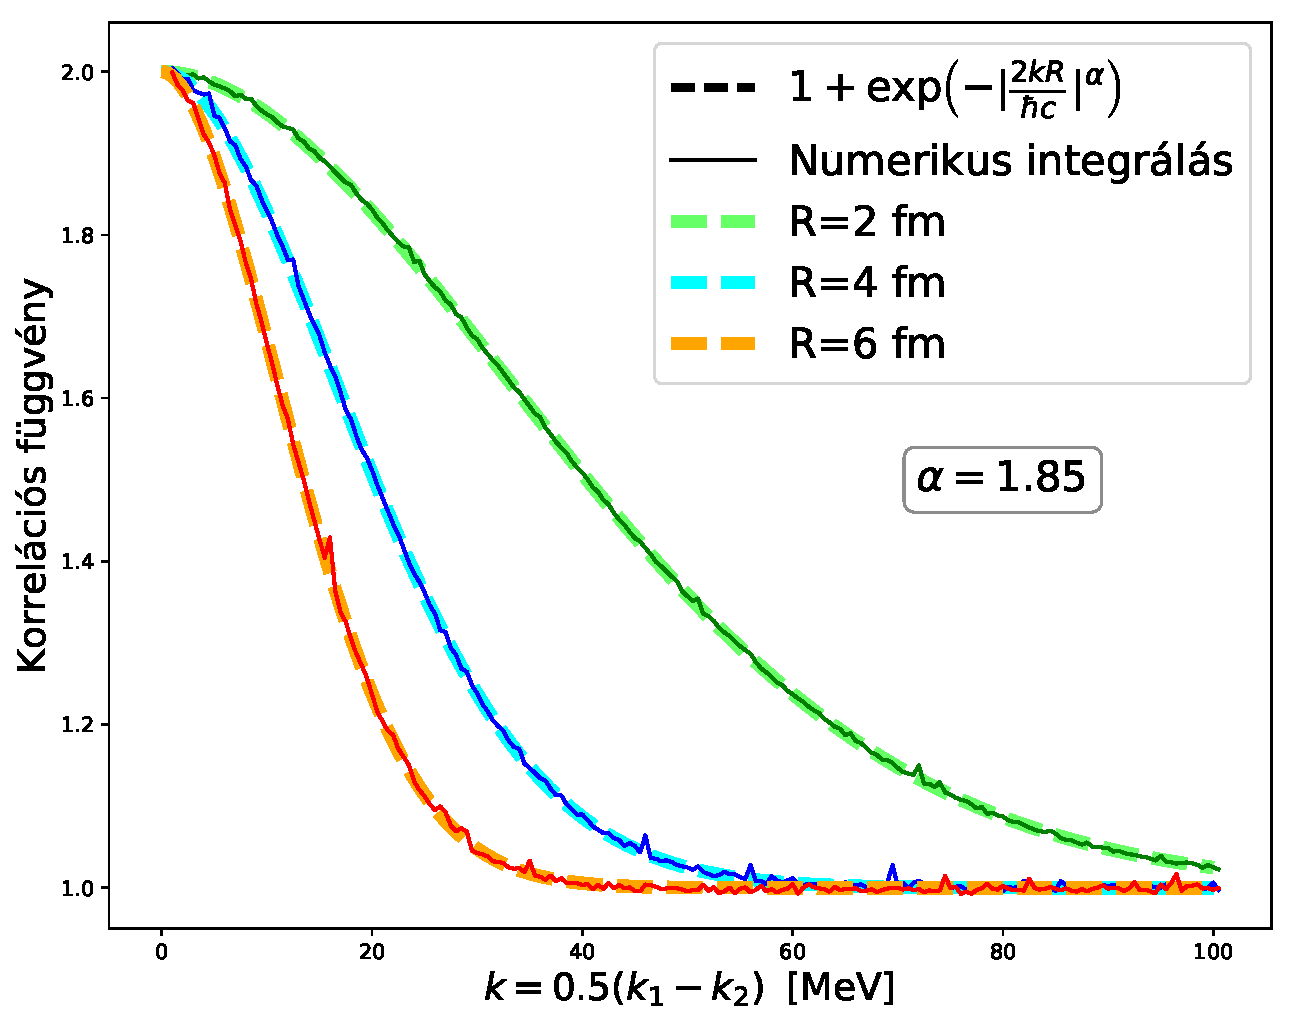
\includegraphics[scale=0.36]{pic/Coulomb/C2_noCoulomb_R246_a185.pdf}
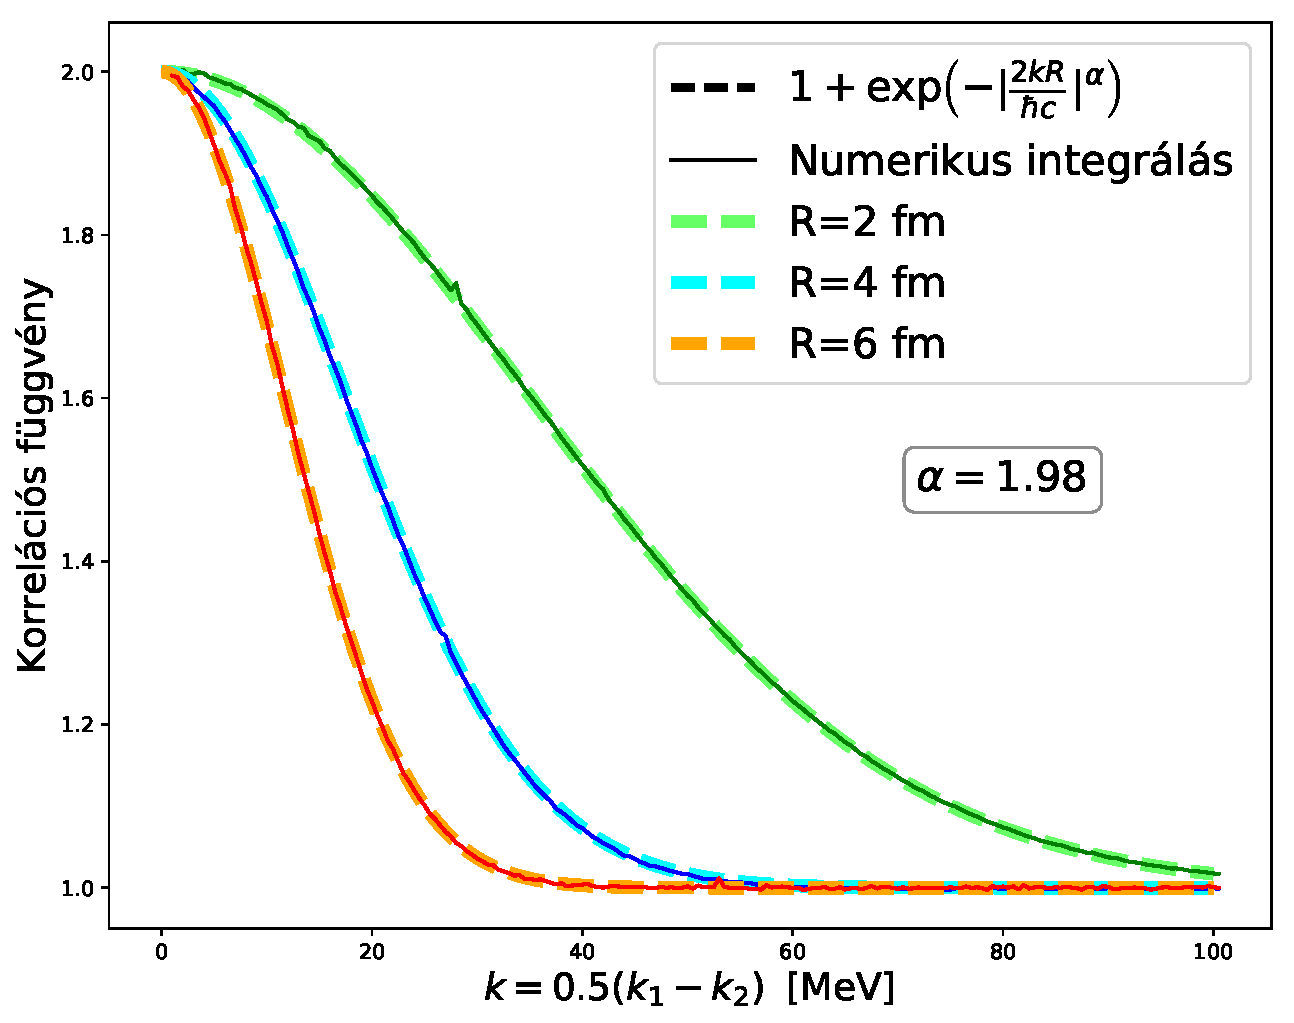
\includegraphics[scale=0.36]{pic/Coulomb/C2_noCoulomb_R246_a198.pdf}
\end{figure}
\begin{figure}[H]
\centering
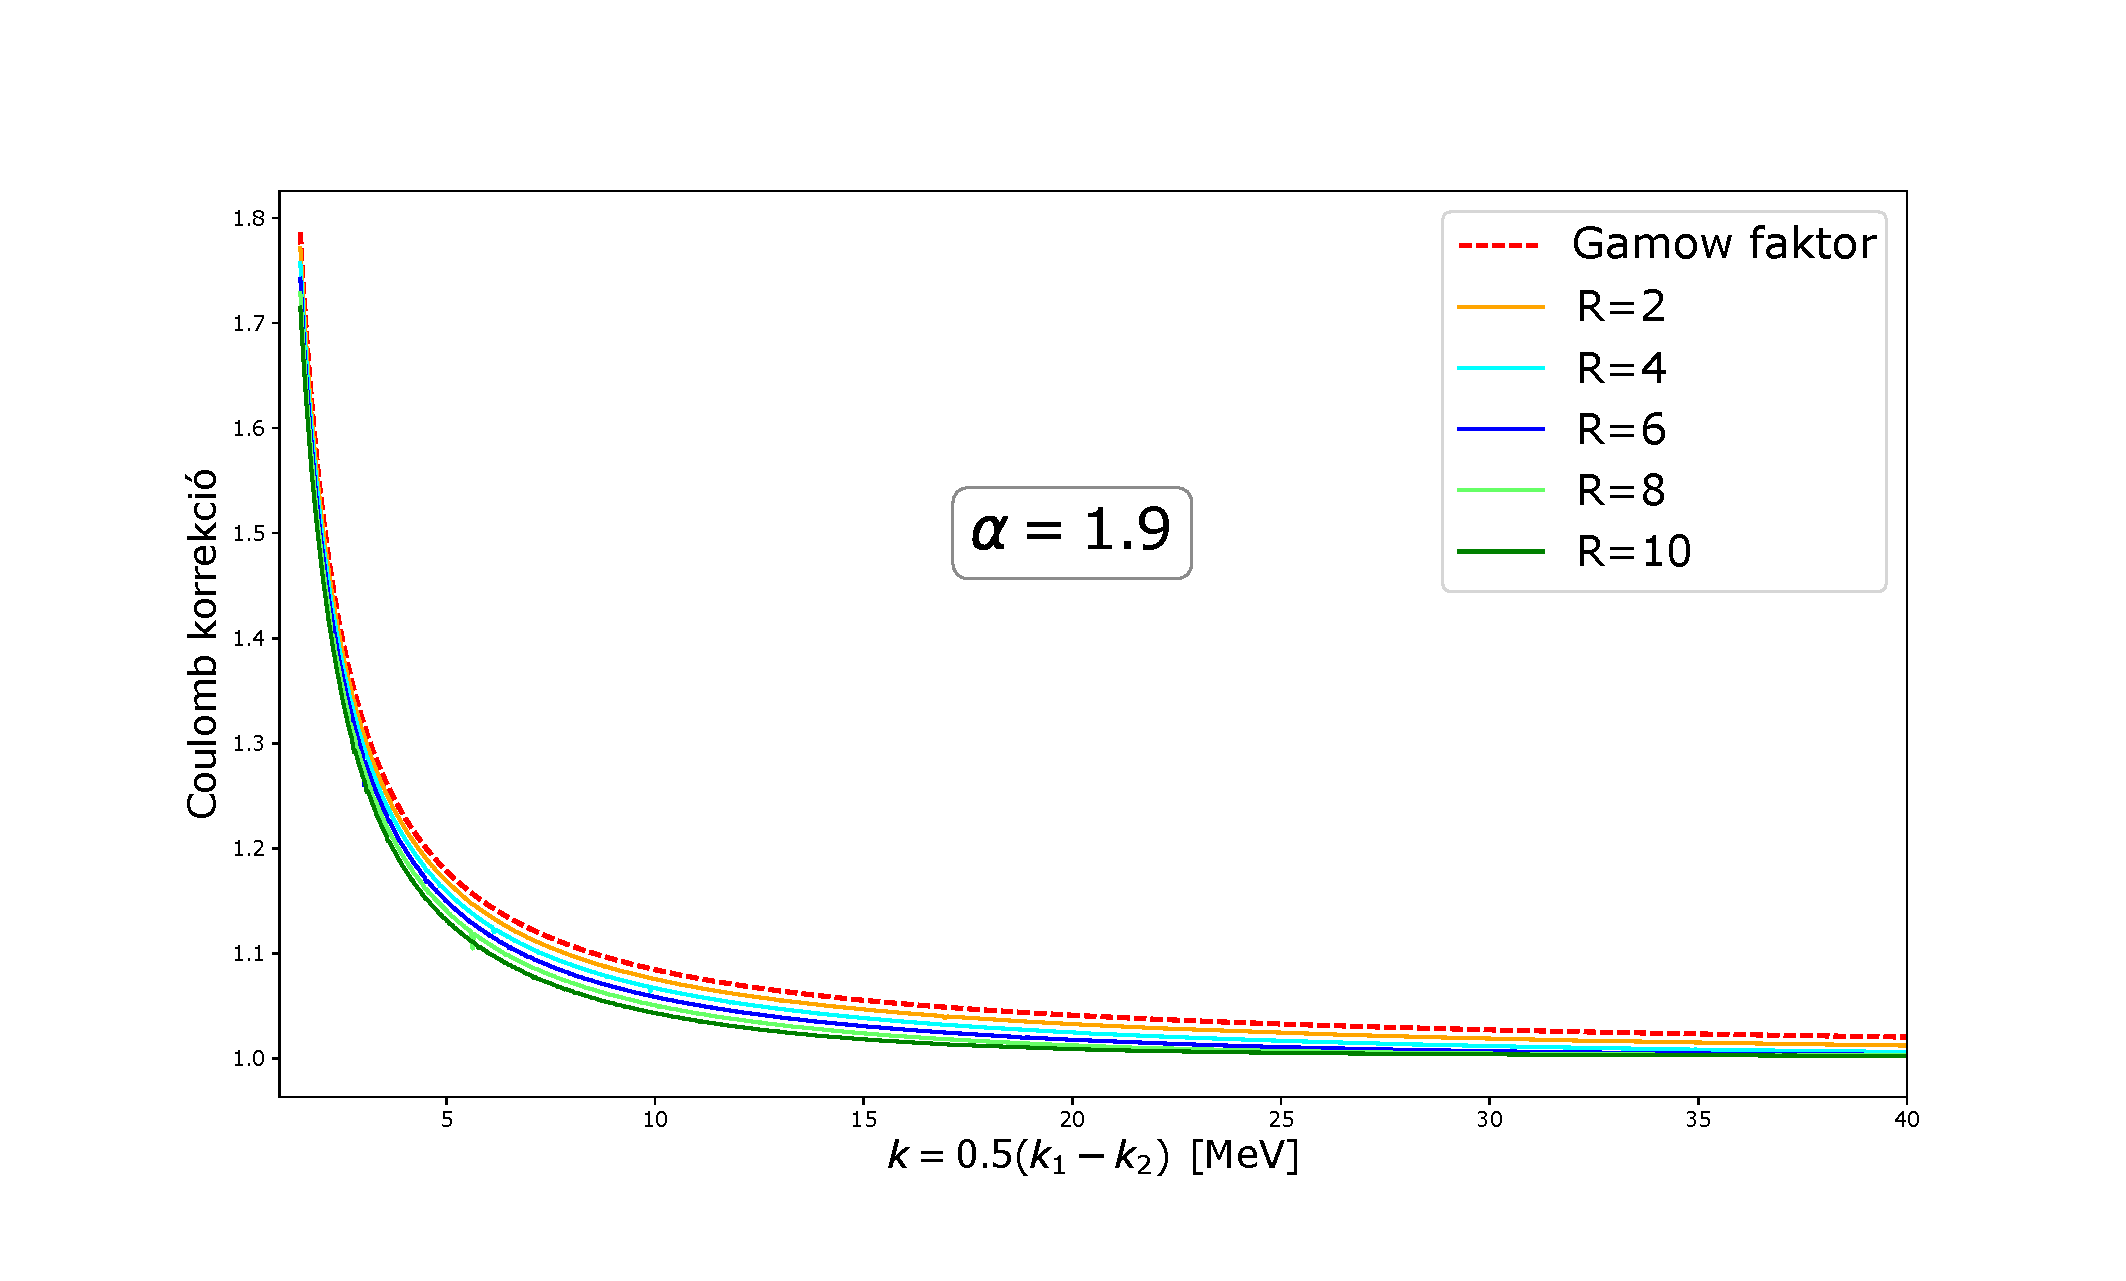
\includegraphics[scale=0.45]{pic/Coulomb/C2_dR_a19_v2.pdf}
\end{figure}
\begin{figure}[H]
\centering
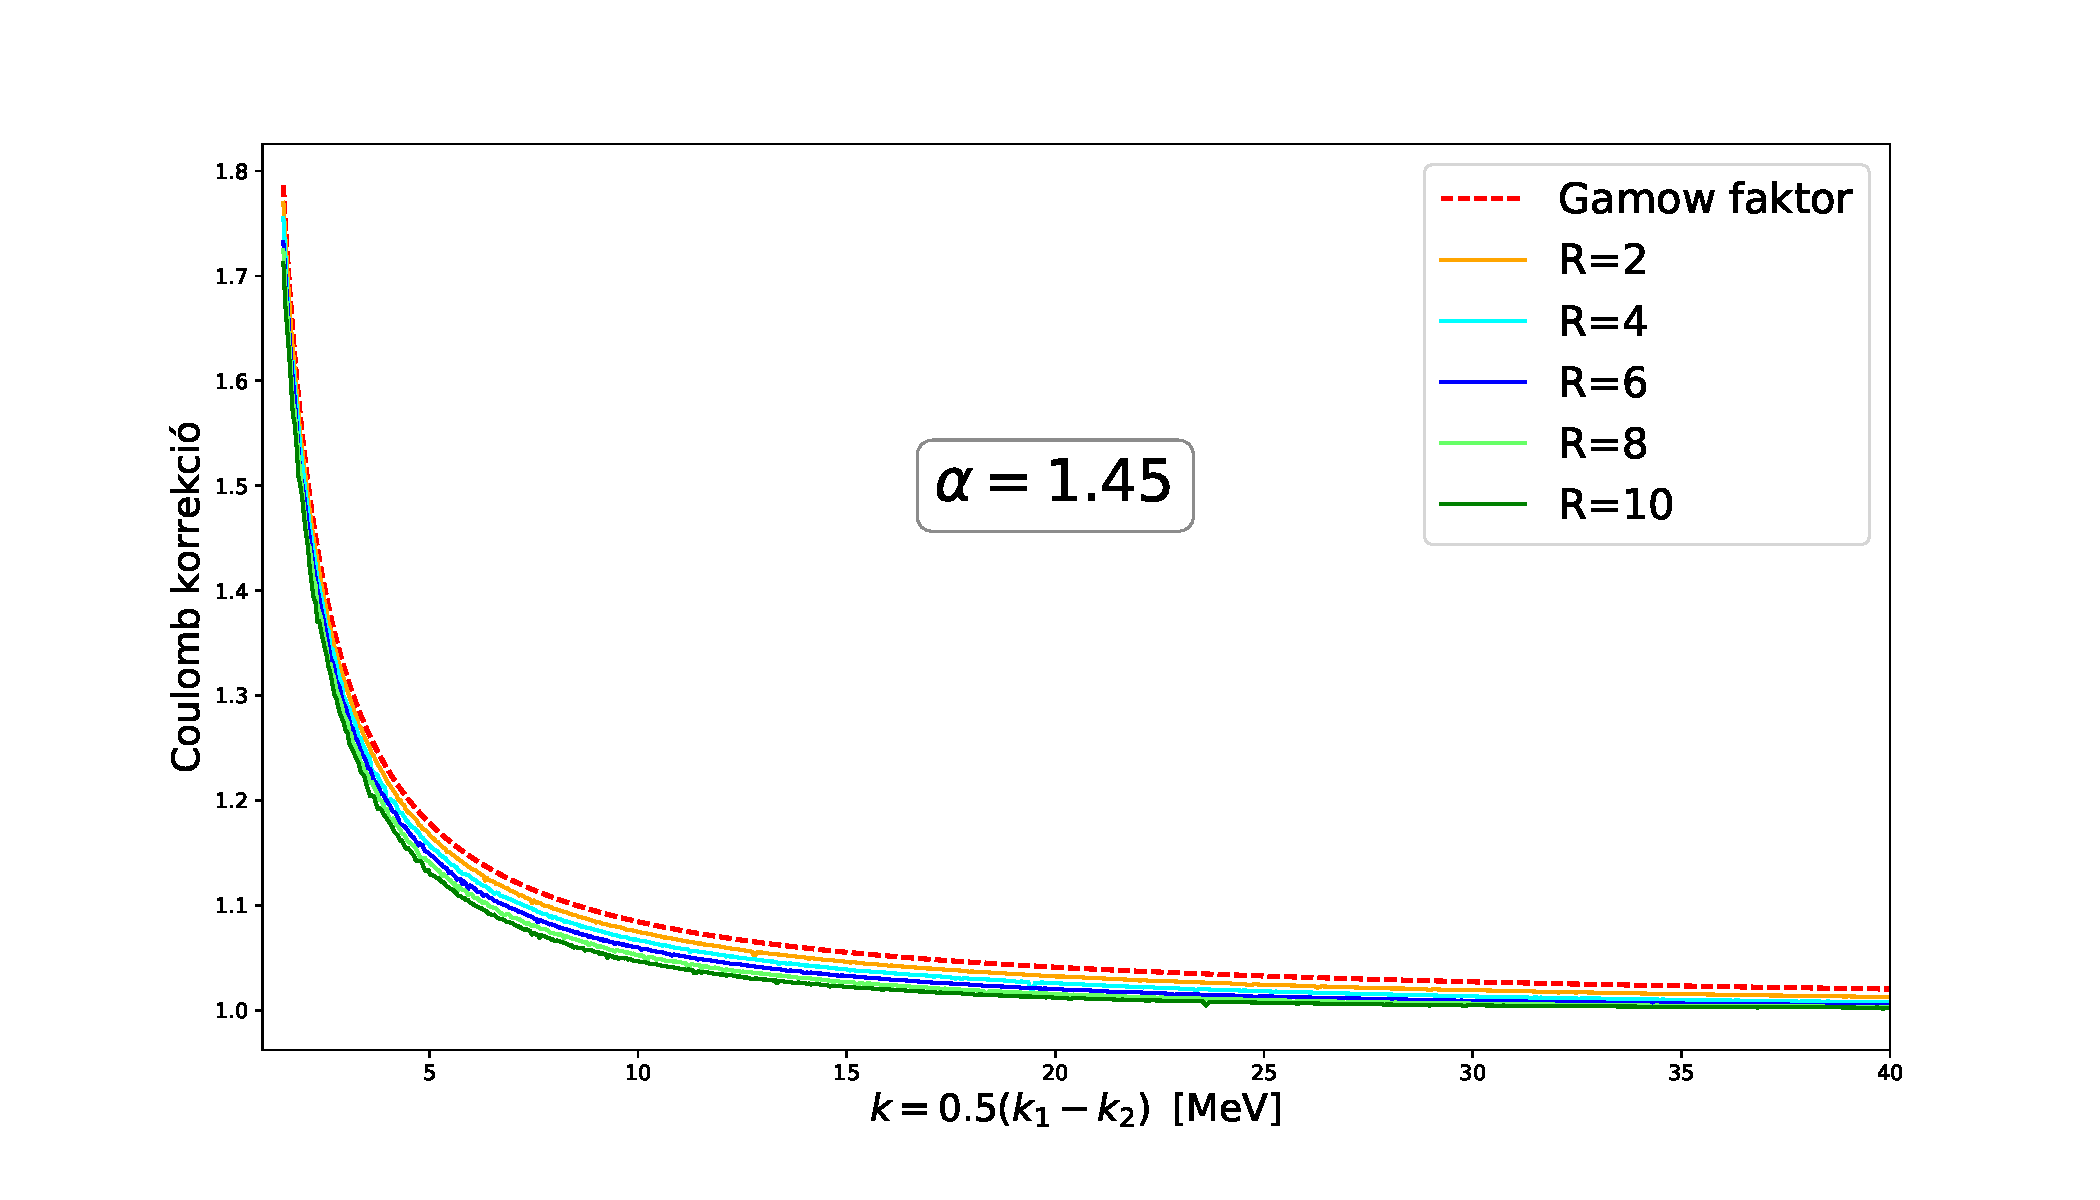
\includegraphics[scale=0.45]{pic/Coulomb/C2_dR_a145.pdf}
\end{figure}

\section{Adatanalízis}
\subsection{Korrelációs függvény változói}
\subsection{Korrelációs függvény mérése}
\subsection{Illesztett modell}

\section{Eredmények}
\subsection{Illesztés vizualizáció}
\begin{figure}[H]
\centering
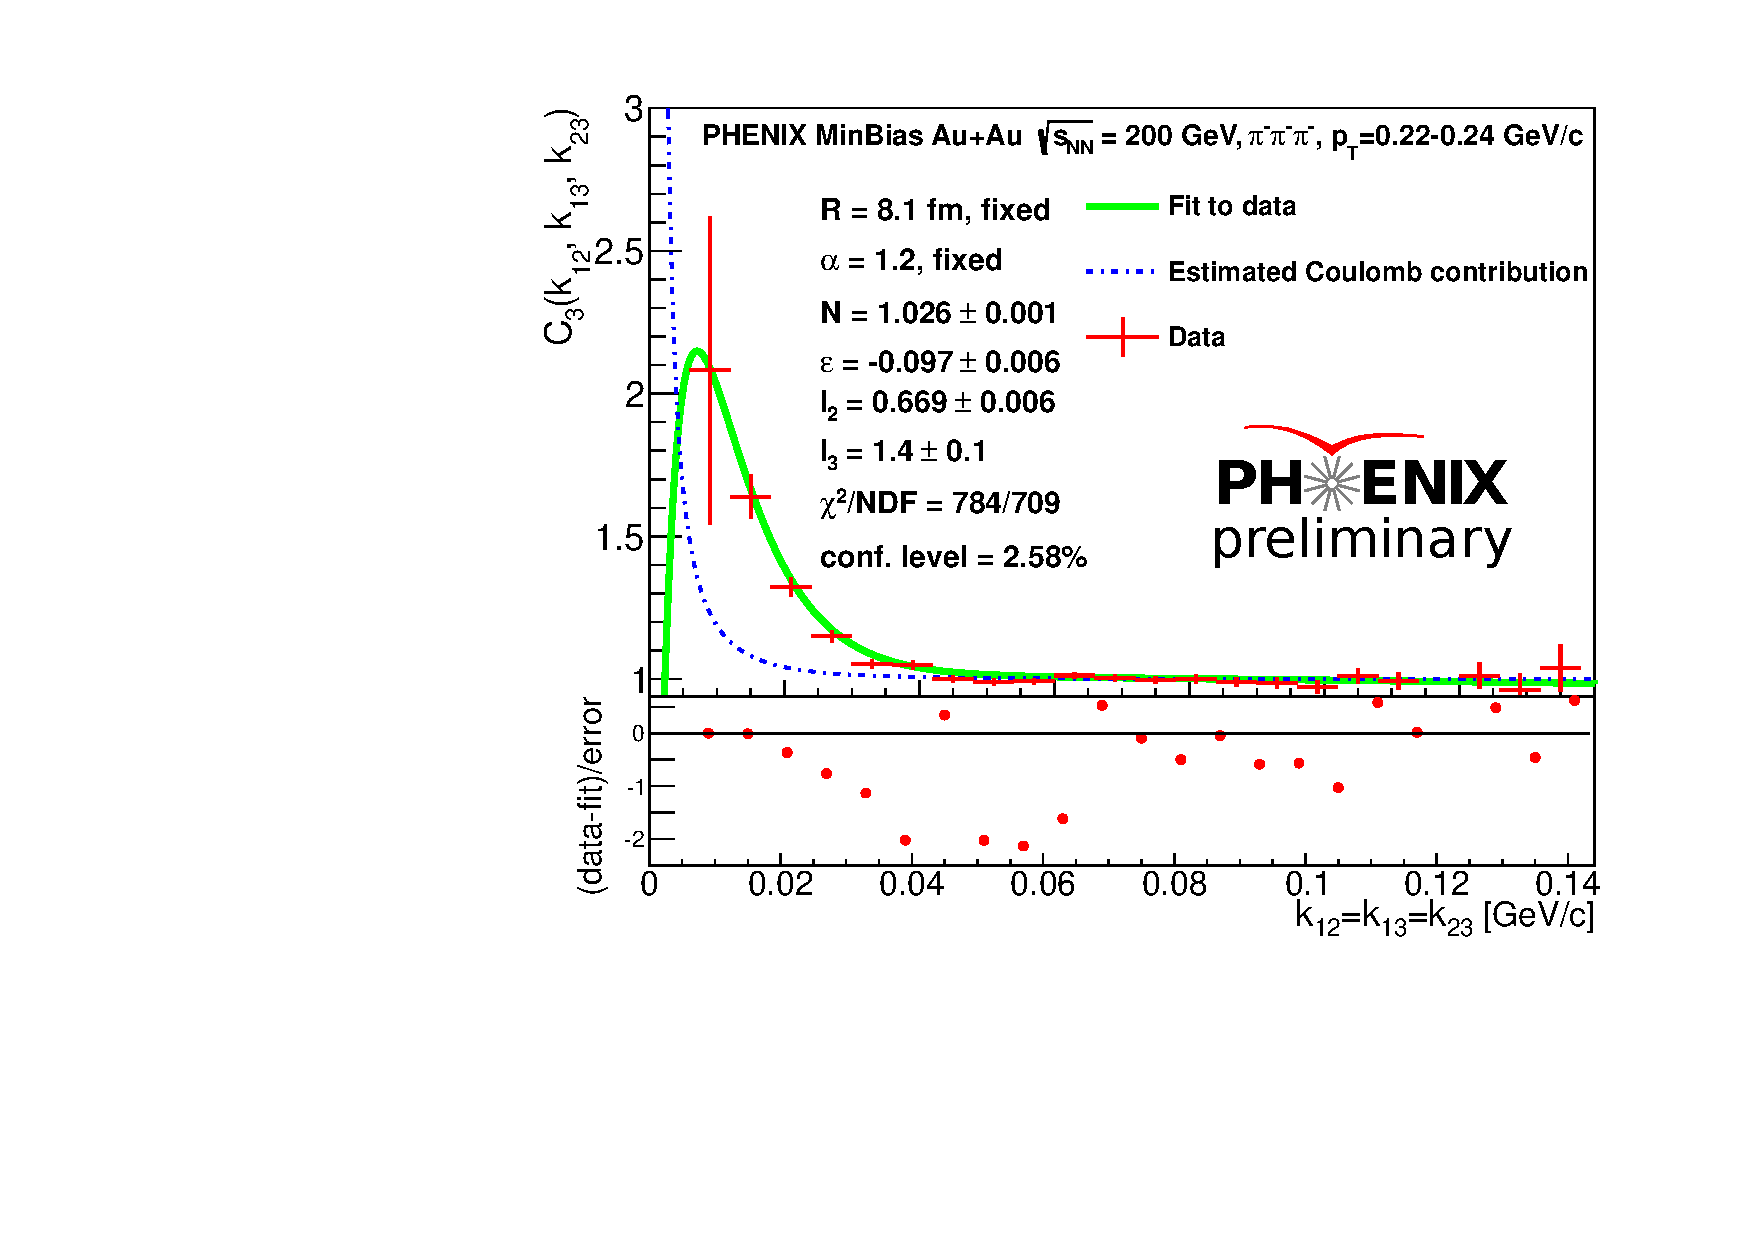
\includegraphics[scale=0.6]{pic/res/diag_lowpt.pdf}
\end{figure}
\begin{figure}[H]
\centering
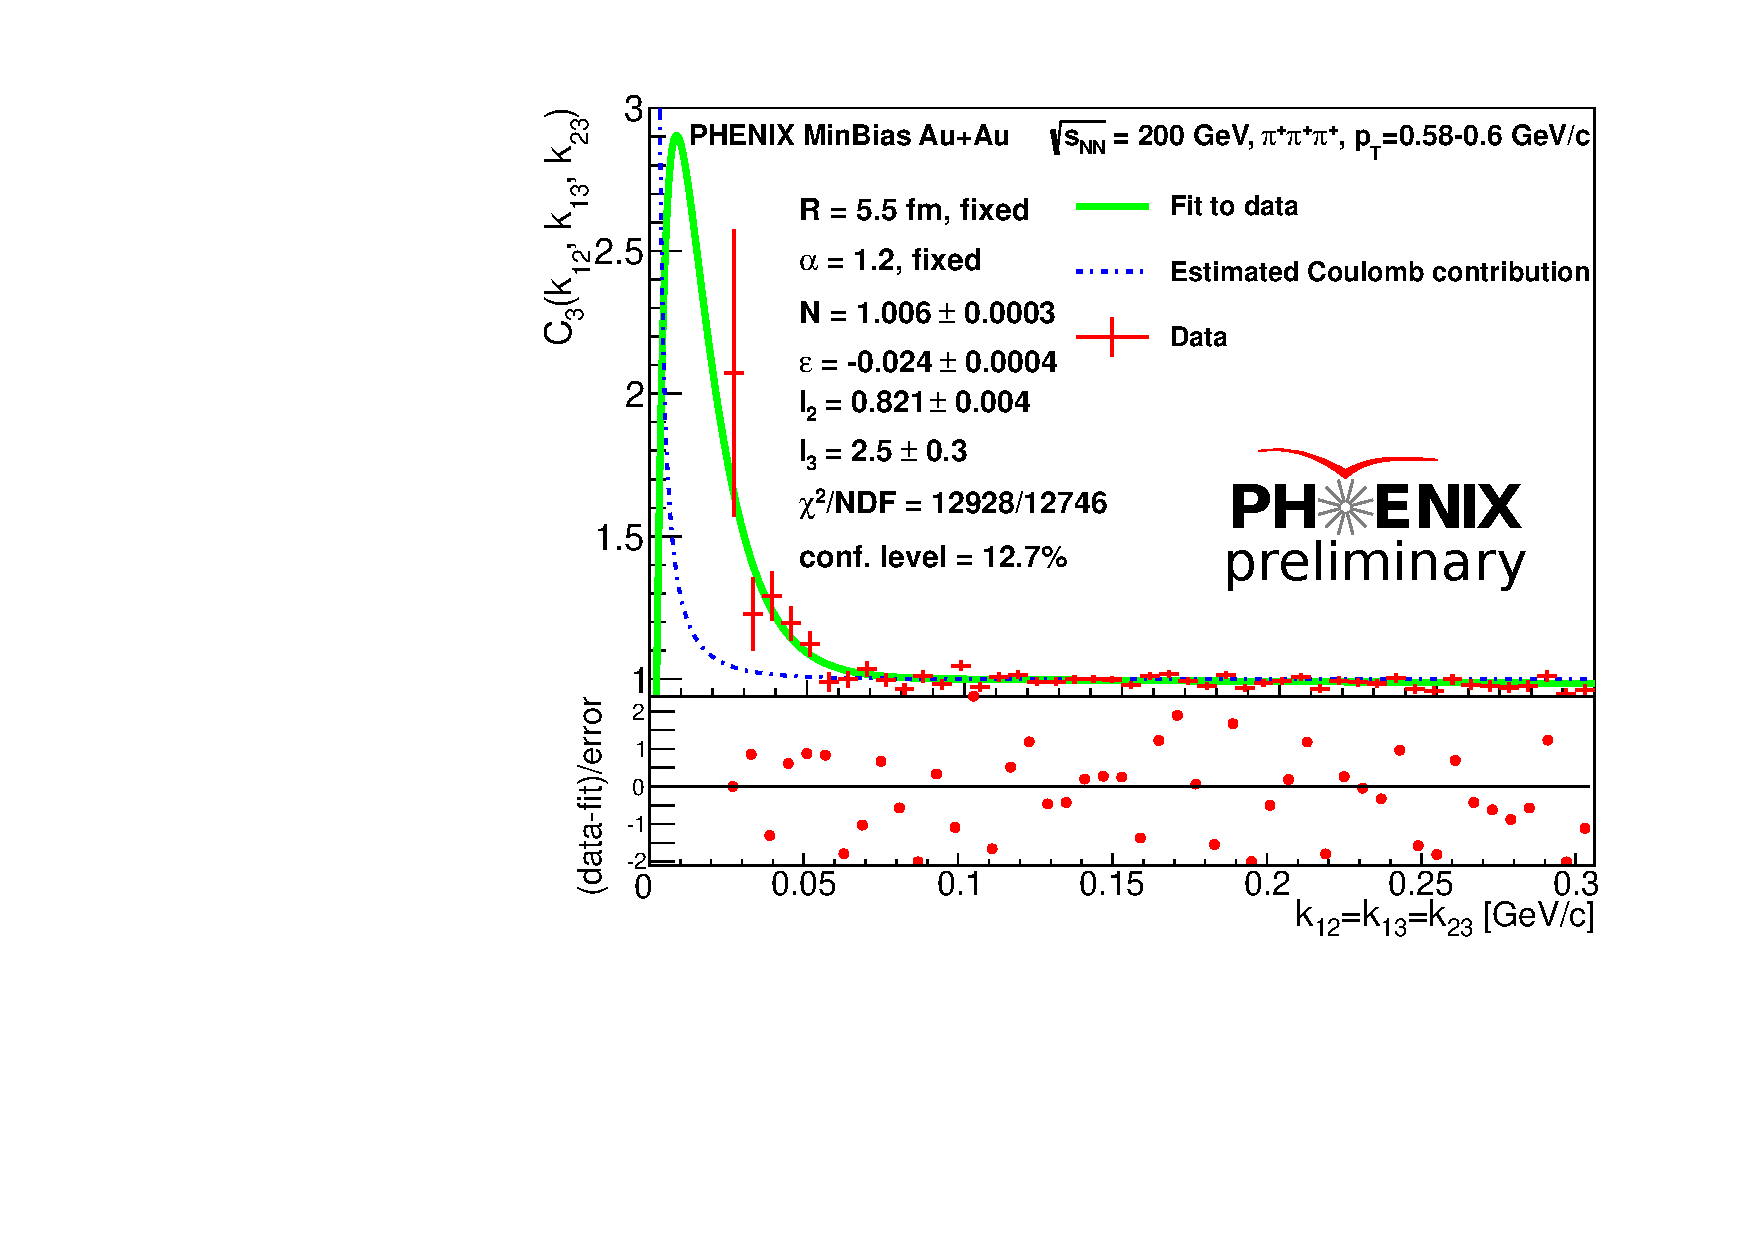
\includegraphics[scale=0.6]{pic/res/diag_highpt.pdf}
\end{figure}
\subsection{Háromrészecske korrelációs erősség}
\begin{figure}[H]
\centering
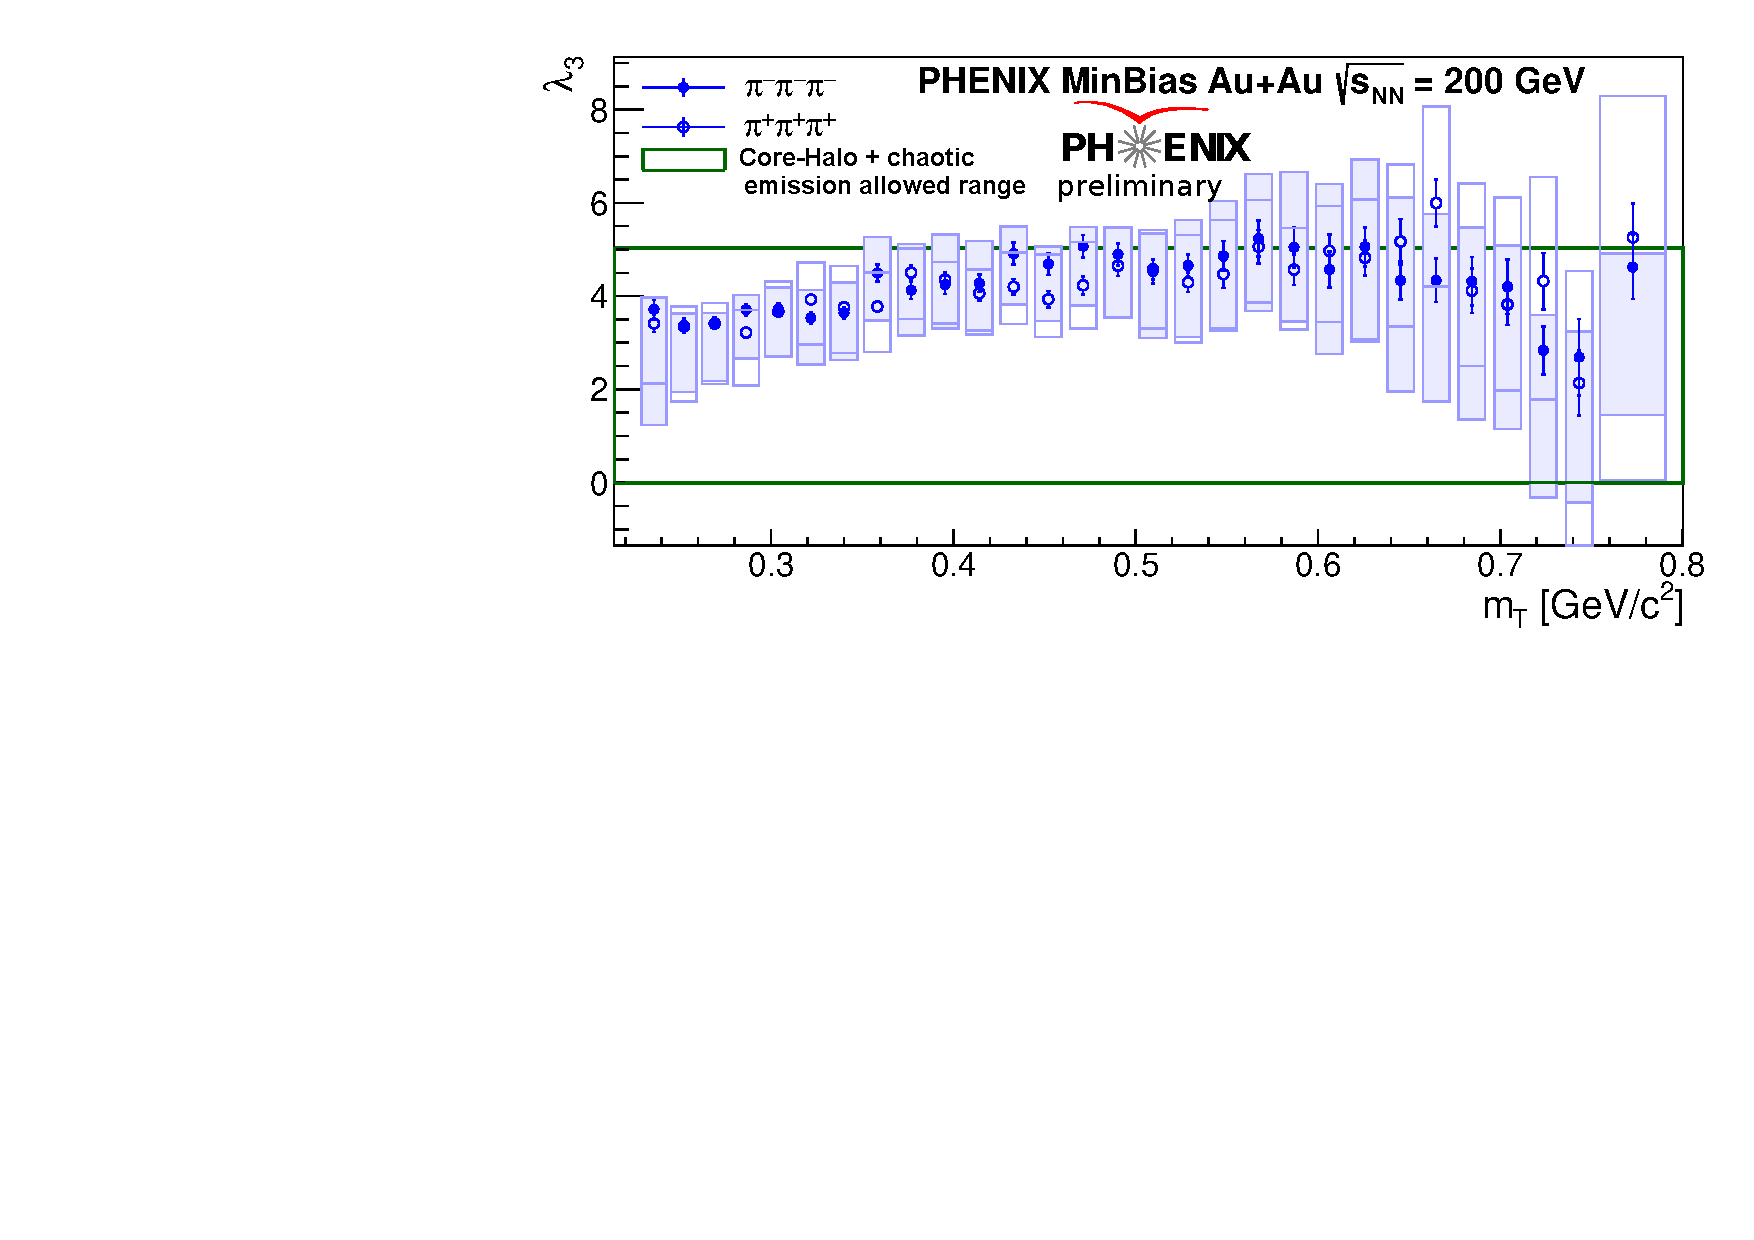
\includegraphics[scale=0.75]{pic/res/lambda3.pdf}
\end{figure}
\subsection{Parciális koherencia}
\begin{figure}[H]
\centering
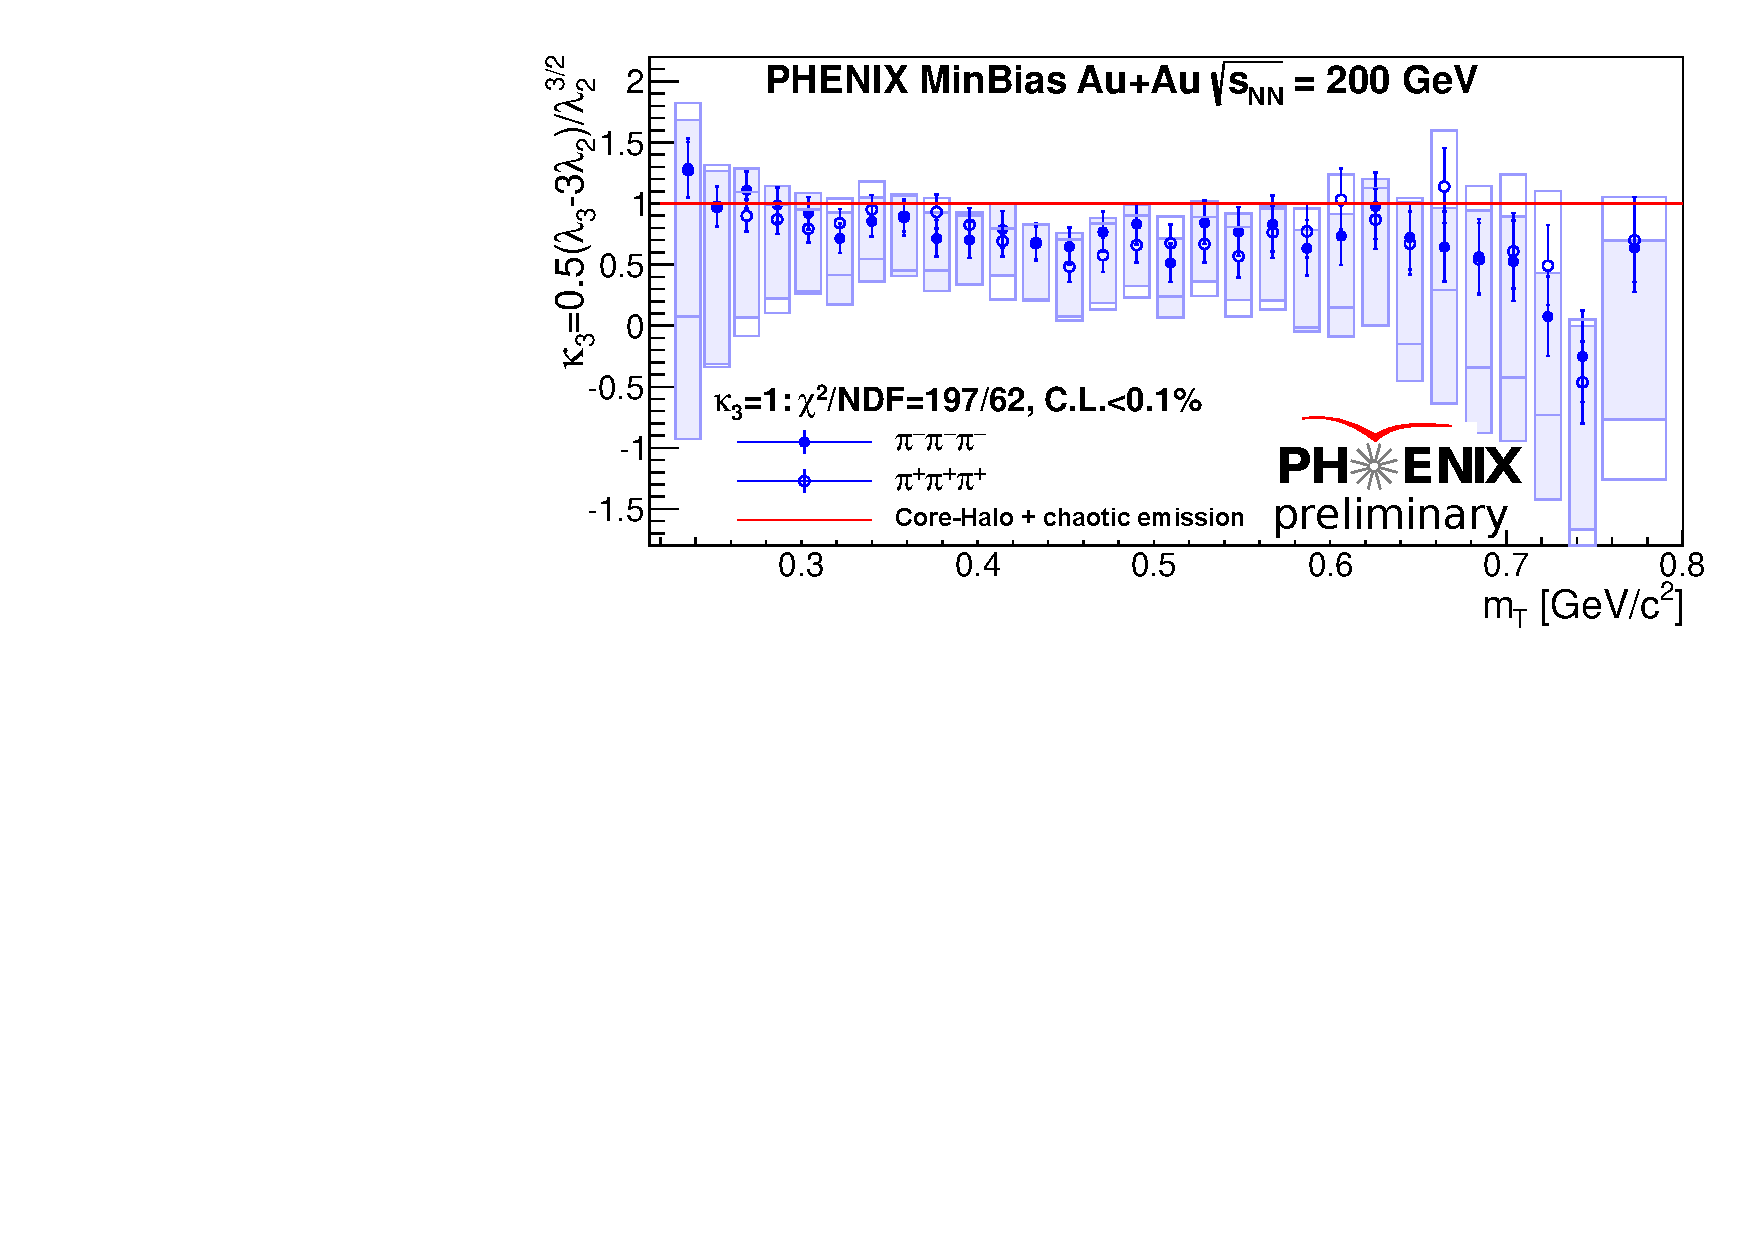
\includegraphics[scale=0.75]{pic/res/kappa3.pdf}
\end{figure}

\begin{figure}[H]
\centering
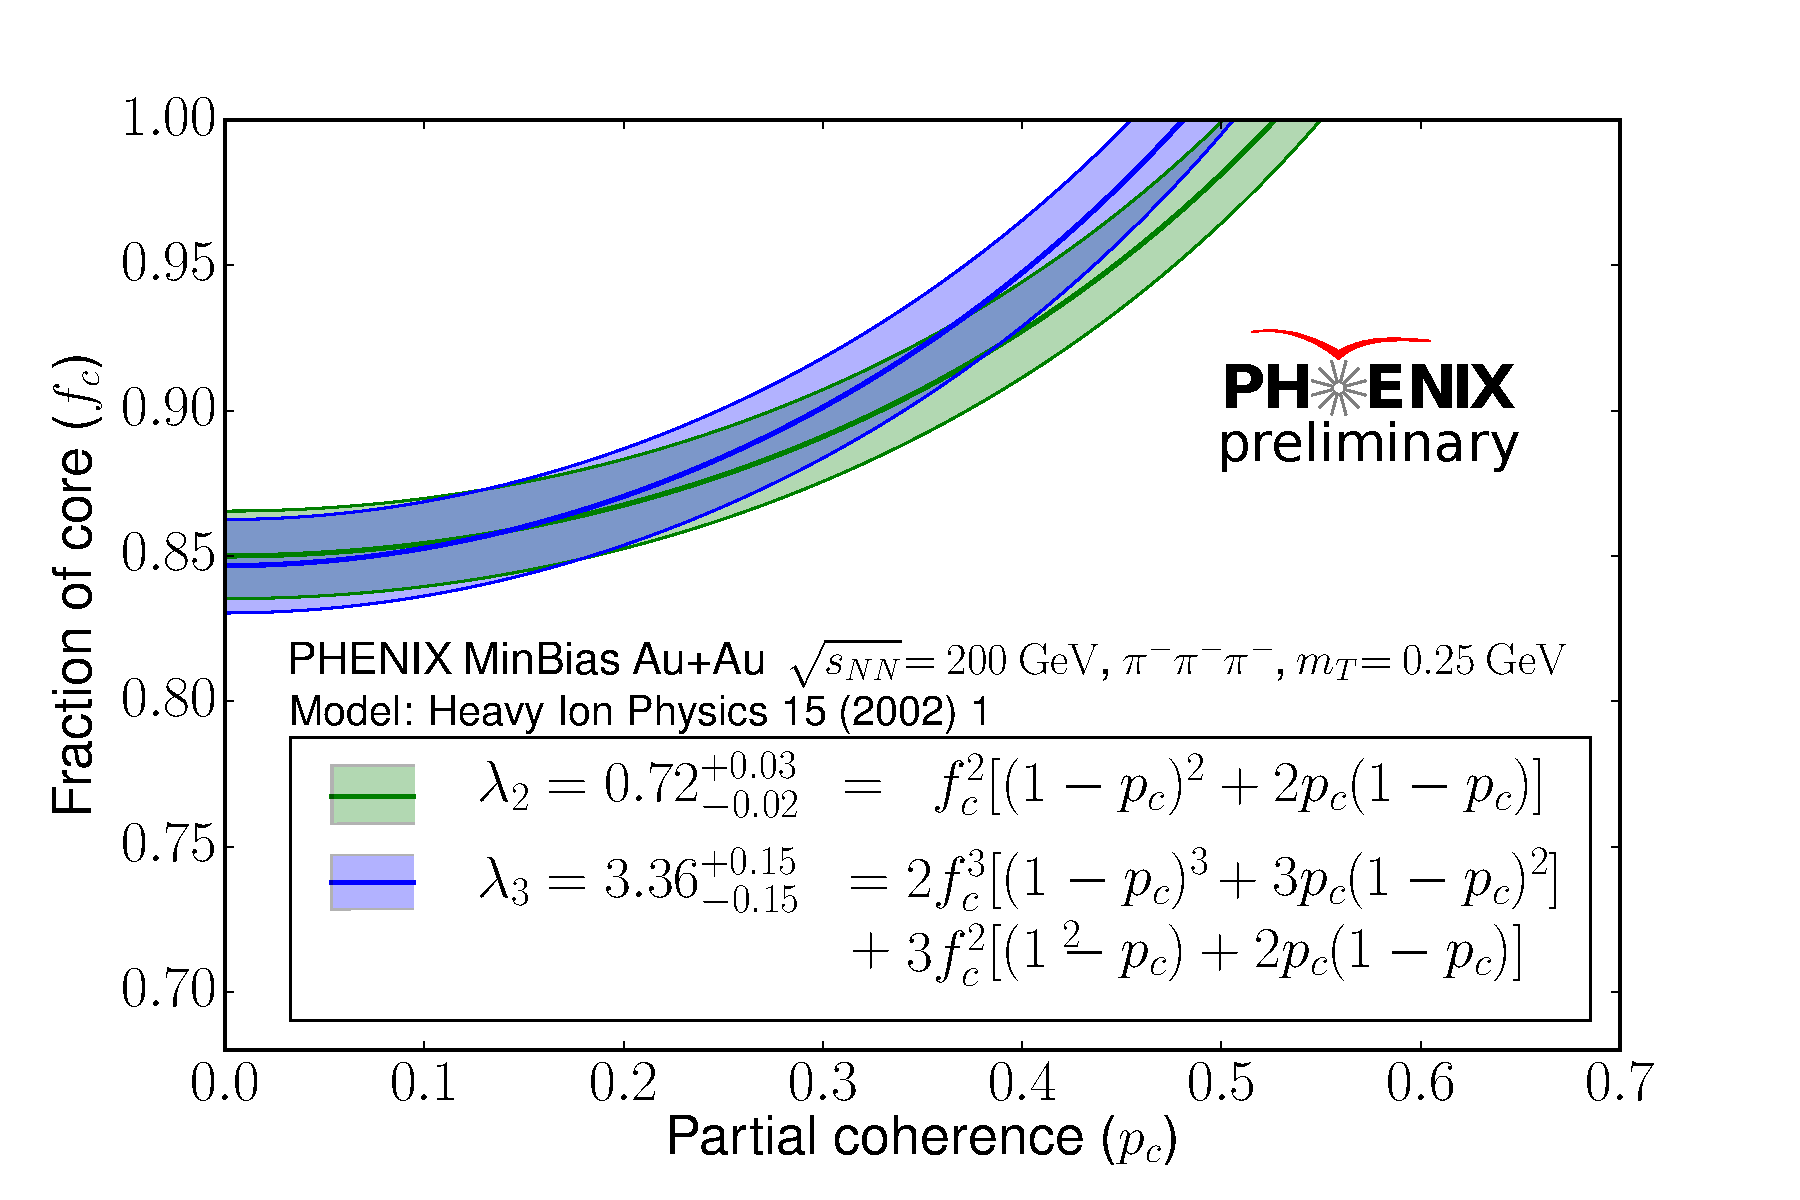
\includegraphics[scale=0.5]{pic/res/fcpc1.pdf}
\end{figure}
\begin{figure}[H]
\centering
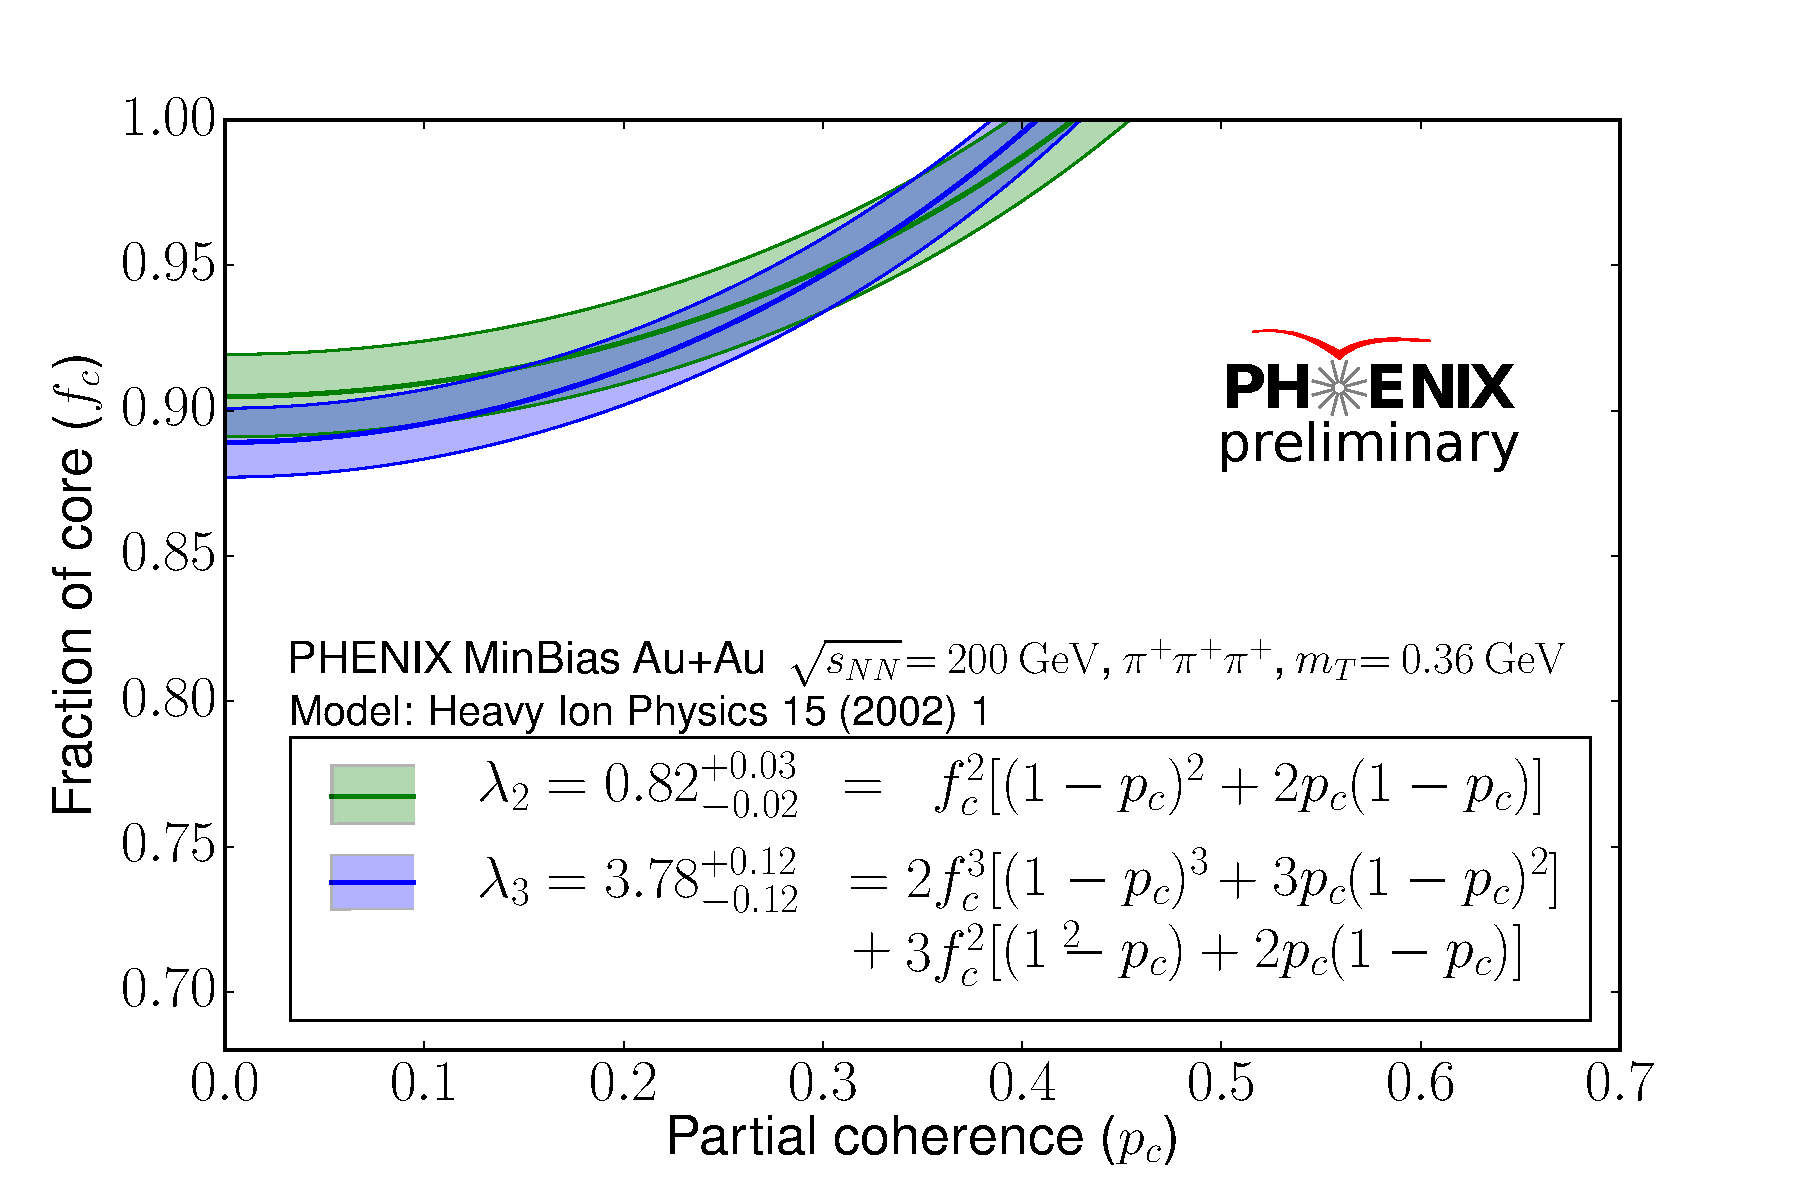
\includegraphics[scale=0.5]{pic/res/fcpc2.pdf}
\end{figure}

\section{Összefoglaló}




\bibliography{ref}

\end{document}
